%% Article SC-Reborn pour International Journal of Production Economics
%% Fichier principal, fondé sur cas-sc-template.tex (Elsevier CAS, une colonne).
%% Le texte de chaque section est dans le dossier sections/.
%% Titre, résumé, points clés et mots-clés : sections/00_front.tex.

\documentclass[a4paper,fleqn]{cas-sc}

\usepackage[T1]{fontenc}
\usepackage[french]{babel}
\usepackage[authoryear,longnamesfirst]{natbib}
\usepackage{amsmath,amssymb}
\usepackage{graphicx}
\usepackage{capt-of} % figures insérées dans le texte, à l'endroit où elles sont citées
\usepackage{tabularx}
\usepackage{enumitem}
\usepackage{tikz}
\usetikzlibrary{arrows.meta,positioning,fit,backgrounds,calc,patterns}
% Couleurs des figures (politiques de gestion et paliers du réseau bayésien)
\definecolor{polnone}{HTML}{5C5B56}
\definecolor{poltard}{HTML}{EDA100}
\definecolor{polprud}{HTML}{EB6834}
\definecolor{polreac}{HTML}{2A78D6}
% Couleurs des politiques dans l'application Isomorph-Reborn
\definecolor{appnone}{HTML}{9CA3AF}
\definecolor{appprud}{HTML}{2563EB}
\definecolor{appreac}{HTML}{DC2626}
\definecolor{apptard}{HTML}{16A34A}
\definecolor{palctx}{HTML}{8A8984}
\definecolor{palpol}{HTML}{2A78D6}
\definecolor{palrep}{HTML}{EDA100}
\definecolor{palmec}{HTML}{1BAF7A}
\definecolor{palres}{HTML}{EB6834}
\usepackage{pgfplots}
\pgfplotsset{compat=1.17}
\newcolumntype{L}{>{\raggedright\arraybackslash}X}
\newcolumntype{P}[1]{>{\raggedright\arraybackslash}p{#1}}
% Champs restant à compléter avant la soumission (en bleu)
\newcommand{\acompleter}[1]{\textcolor{blue}{#1}}

% Mettre \anonymetrue pour la version soumise en double aveugle (masque auteurs, affiliations, CRediT et financement).
\newif\ifanonyme
\anonymefalse
% \anonymetrue

% Titre, points clés et mots-clés (rapatriés du doc de travail).
% Le résumé est écrit directement dans sc_reborn_ijpe.tex : la classe le recopie
% mot pour mot dans un fichier et n'accepte pas de macro.
\newcommand{\ArticleTitle}{Jumeau numérique et pilotage bayésien causal de la résilience des chaînes logistiques}
\newcommand{\ArticleHighlights}{\item Des crises simulées relient perturbation, décision et trajectoire de performance
\item Le rejeu contrefactuel isole l'effet de la réaction managériale
\item Une courbe à sept paramètres traduit le service en six indicateurs de résilience
\item Un réseau bayésien causal diagnostique et pronostique la résilience
\item Réagir tôt raccourcit la crise et rentabilise chaque levier engagé}
\newcommand{\ArticleKeywords}{résilience des chaînes logistiques \sep gestion des perturbations \sep réseaux bayésiens \sep inférence causale \sep simulation \sep courbe de résilience \sep aide à la décision}


\begin{document}
\let\WriteBookmarks\relax
\def\floatpagepagefraction{1}
\def\textpagefraction{.001}

\shorttitle{Résilience des réseaux logistiques : simuler, mesurer, apprendre}
\ifanonyme\shortauthors{Auteurs anonymisés}\else\shortauthors{N. Rahiel et al.}\fi

\title [mode = title]{\ArticleTitle}

\ifanonyme
\author[1]{\acompleter{Auteurs anonymisés pour l'évaluation}}
\affiliation[1]{organization={\acompleter{Anonymisé}},
            country={France}}
\else
\author[1]{Naïma Rahiel}
\author[1]{Sid-Ali Addouche}
\cormark[1]
\author[1]{El Mouloudi Dafaoui}
\author[1]{Abderrahman El Mhamedi}
\author[2,3]{Saïd Amari}
\author[4]{Agnès Letouzey}
\author[4]{Xavier Desforges}
\author[4]{Kamal Medjaher}
\affiliation[1]{organization={Laboratoire QUARTZ, IUT de Montreuil, Université Paris 8},
            city={Montreuil},
            country={France}}
\affiliation[2]{organization={LURPA, ENS Paris-Saclay},
            city={Gif-sur-Yvette},
            country={France}}
\affiliation[3]{organization={LIPN, Université Sorbonne Paris Nord},
            city={Villetaneuse},
            country={France}}
\affiliation[4]{organization={LGP, Université de Toulouse, UTTOP},
            city={Tarbes},
            country={France}}
\cortext[1]{Auteur correspondant}
\fi

\begin{abstract}
La résilience d'une chaîne logistique dépend autant de la réaction des gestionnaires que de la perturbation elle-même. Pourtant, aucune base de données ne relie une perturbation, les décisions prises et la trajectoire de performance qui en résulte. Nous proposons une démarche en trois étapes. Premièrement, un réseau logistique multi-échelon est soumis à des perturbations maîtrisées de cinq natures, tandis qu'un gestionnaire simulé détecte la dégradation, décide et escalade parmi neuf leviers ; chaque crise est rejouée sans réaction et sous trois profils de gestionnaire, de sorte que les écarts de performance sont attribuables à la seule gestion. Deuxièmement, chaque trajectoire de service est résumée par une courbe de résilience hyperbolique composée, dont six indicateurs sont déduits analytiquement. Troisièmement, un réseau bayésien causal, dont la structure suit l'ordre temporel d'une crise et traite la politique de gestion comme une intervention, en tire pronostic, diagnostic et préconisation. Sur 2 000 crises simulées sur le réseau d'un jumeau numérique ouvert, la réaction agit sur la durée de la crise plutôt que sur sa profondeur : la politique la plus réactive évite 73 \% du service perdu, contre 18 \% et 14 \% pour les politiques prudente et tardive. Chaque levier qu'elle engage préserve en moyenne un tiers de journée de ventes, alors que la politique prudente est économiquement dominée. Le réseau appris préconise, lorsque la durée du choc est connue, une politique plus sobre dans environ une crise sur sept sans perte notable de résilience.
\end{abstract}

\begin{highlights}
\ArticleHighlights
\end{highlights}

\begin{keywords}
\ArticleKeywords
\end{keywords}

\maketitle

% Rapatrié depuis le doc de travail (onglet Article FR), révision 144.

\section{Introduction}
\label{sec:1}

Les chaînes logistiques sont exposées à des perturbations dont les effets durent plusieurs semaines : défaillances de fournisseurs, coupures de liaisons de transport, fermetures de sites, pics de demande ou congestion généralisée. Leurs conséquences économiques, ventes perdues, pénalités contractuelles, transports d'urgence et heures supplémentaires, dépendent non seulement de la sévérité du choc, mais aussi de la rapidité et de la pertinence de la réaction des gestionnaires \citep{sheffi2005book,ivanov2019ijpr}. La robustesse, capacité à absorber un choc sans dégradation, ne suffit donc pas ; la résilience, capacité à limiter la perte et à se rétablir, dépend largement des décisions prises pendant la crise.

La littérature offre une typologie riche des stratégies d'atténuation et de contingence \citep{tomlin2006,chopra2004} et une représentation bien établie de la résilience sous forme de courbe de perte et de rétablissement, le triangle de résilience \citep{bruneau2003}. Les gestionnaires manquent pourtant d'outils d'aide à la décision capables de répondre à deux questions pratiques : face à une perturbation donnée, quelle politique de réaction a le plus de chances d'atteindre un niveau de résilience visé, et, après un rétablissement médiocre, était-ce le choc, le réseau ou la réaction qui était en cause ? Y répondre exige des observations reliant une perturbation, les décisions prises et la trajectoire de performance qui en résulte. De telles données sont rares : les données d'entreprise sont confidentielles et incomplètes, les bases publiques décrivent les perturbations à un niveau macroéconomique sans les décisions, et les études par simulation ne rapportent qu'un petit nombre de cas agrégés \citep{ramzy2022,do2024}.

Cet article propose une démarche en trois étapes pour combler ce manque (Fig.~\ref{fig:d1}). La première génère par simulation des scénarios de crise étiquetés. Un réseau logistique multi-échelon, par exemple le réseau d'origine du jumeau numérique ouvert ISOMORPH \citep{zhang2026isomorph}, représenté par ses seules capacités ou avec ses délais et ses stocks, est soumis à des perturbations maîtrisées, un gestionnaire simulé y réagit, et chaque crise est rejouée sans réaction et sous trois profils de gestionnaire. La deuxième caractérise chaque trajectoire journalière de service par l'ajustement d'une courbe de résilience à sept paramètres et en déduit six indicateurs de résilience. La troisième apprend, à partir de la base obtenue, un réseau bayésien causal \citep{pearl2009} qui permet le pronostic, le diagnostic et la préconisation de politiques de gestion.

\begin{figure*}[htbp]
\centering
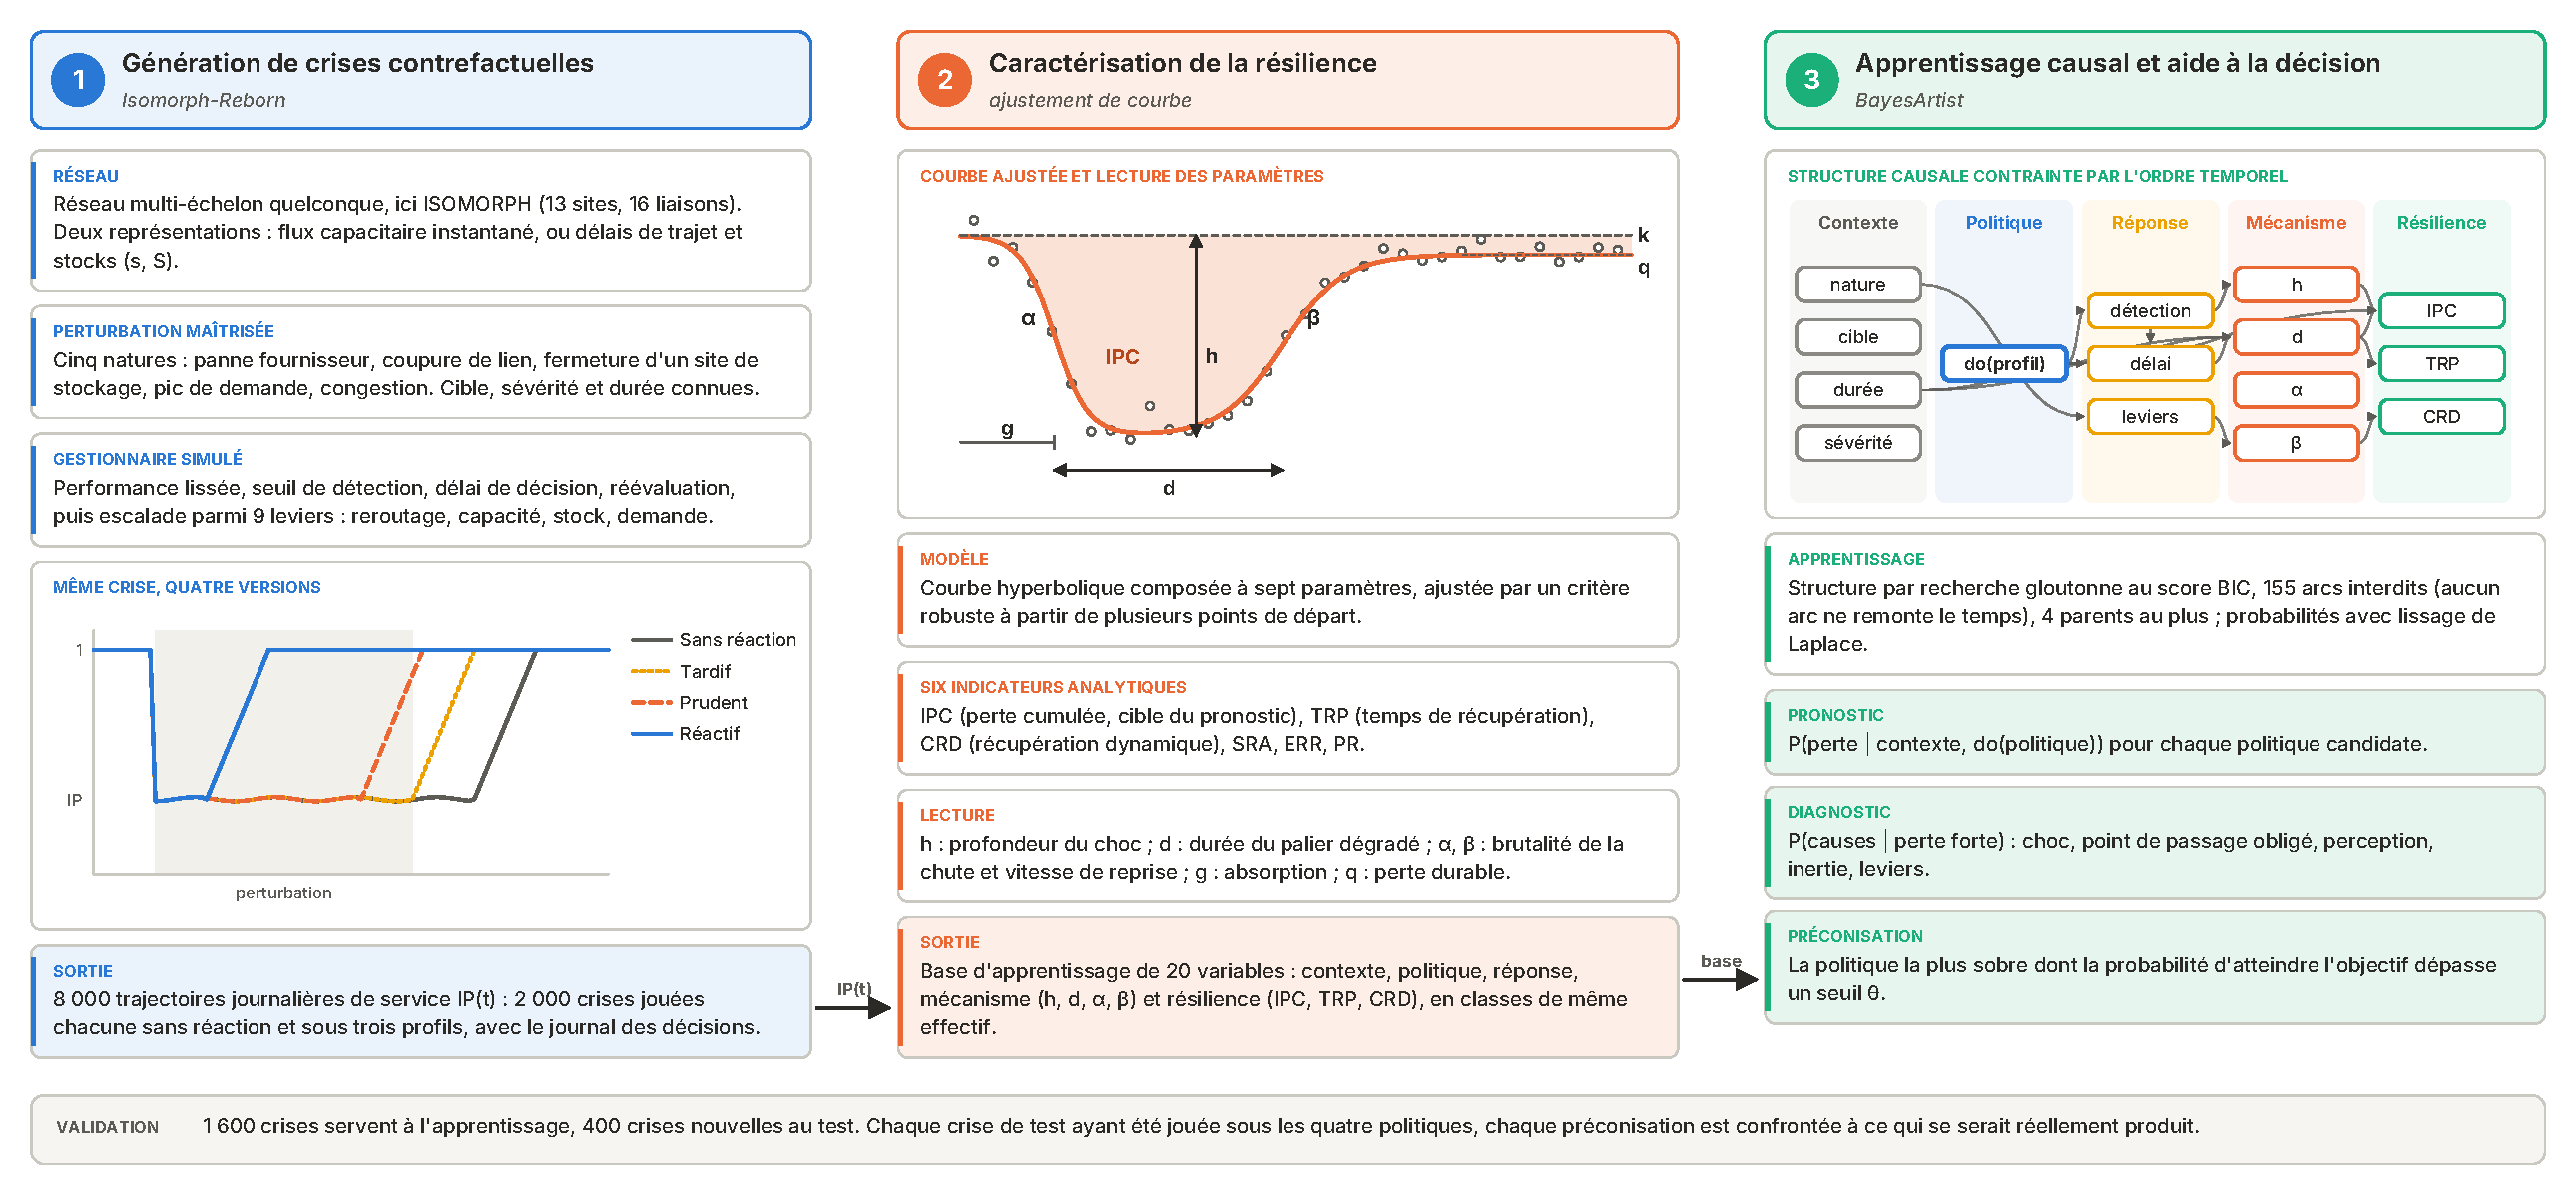
\includegraphics[width=\textwidth]{figures/Fig1_demarche.pdf}
\caption{Démarche en trois blocs. Le bloc 1 joue chaque crise sous quatre politiques de gestion ; le bloc 2 résume chaque trajectoire par une courbe à sept paramètres et six indicateurs ; le bloc 3 apprend un réseau bayésien dont la structure respecte l'ordre temporel d'une crise, et en tire pronostic, diagnostic et préconisation.}
\label{fig:d1}
\end{figure*}

La contribution est triple. D'abord, un générateur de scénarios produisant des crises étiquetées par leur cause exacte et rejouées de manière contrefactuelle, ce qui sépare l'effet de la gestion de celui de la perturbation ; applicable à un réseau multi-échelon quelconque, il fait de la couverture de stock un facteur d'étude plutôt qu'un obstacle. Ensuite, une caractérisation paramétrique de la résilience dont les paramètres ont une lecture opérationnelle directe, reliant la forme d'une crise aux mécanismes de dysfonctionnement. Enfin, un modèle causal dont la structure suit l'ordre temporel d'une crise et traite la politique de gestion comme une intervention, ce qui rend son effet sur la résilience identifiable.

La suite de l'article est organisée comme suit. La section 2 présente l'état de l'art. Les sections 3, 4 et 5 décrivent les trois étapes de la démarche. La section 6 présente les résultats, la section 7 discute les apports, les implications managériales et les limites, et la section 8 conclut.

% =====================================================================
% Section 2 : État de l'art
% Rédaction du 6 octobre 2026. Chaque citation a été vérifiée (DOI) ;
% les articles comparés directement à notre travail ont été lus en entier
% ou, à défaut, cités pour ce qu'affirme leur résumé.
% Les renvois aux sections 3 à 6 et à la figure 1 sont écrits en dur
% tant que le reste de l'article n'est pas rapatrié dans ce dépôt.
% =====================================================================

\section{État de l'art}
\label{sec:etat}

La résilience d'un réseau logistique se lit dans la façon dont sa performance se dégrade puis se rétablit après une perturbation. Cette trajectoire dépend de deux facteurs : ce qui a frappé le réseau et ce que le gestionnaire a décidé pour y répondre. Préconiser une décision suppose donc de relier, pour un grand nombre de crises, la perturbation subie, la décision prise et la trajectoire qui en résulte. Cette section examine comment la littérature traite chacun de ces éléments : la mesure de la résilience (section~\ref{sec:ea-mesure}), les stratégies d'atténuation et de contingence (section~\ref{sec:ea-strategies}), la simulation des perturbations et du rétablissement (section~\ref{sec:ea-simulation}) et les réseaux bayésiens causaux (section~\ref{sec:ea-rb}). La section~\ref{sec:ea-lacune} en tire le manque que ce travail vise à combler.

% ---------------------------------------------------------------------
\subsection{Résilience des chaînes logistiques : définitions, courbe et triangle de résilience}
\label{sec:ea-mesure}

Les revues de littérature s'accordent sur une définition de la résilience comme la capacité d'une chaîne logistique à se préparer aux perturbations, à y répondre et à s'en rétablir \citep{tukamuhabwa2015, kamalahmadi2016}. \citet{kamalahmadi2016} organisent cette capacité en trois phases, l'anticipation, la résistance, puis le rétablissement et la réponse. Leur revue de cent articles montre aussi que la mesure reste le parent pauvre du domaine : huit travaux seulement y sont consacrés, contre soixante-huit aux principes de la résilience. Une partie des mesures existantes repose sur la perception des acteurs, comme l'échelle de \citet{chowdhury2017}, qui évalue par enquête les capacités proactive et réactive et la qualité de conception de la chaîne. Ces mesures renseignent sur les capacités d'une entreprise, mais pas sur ce qui se passe pendant une crise donnée.

L'autre famille de mesures part de la performance observée dans le temps. \citet{bruneau2003} associent la perte de résilience à la surface comprise entre la performance nominale et la performance dégradée, jusqu'au retour à l'équilibre : c'est le triangle de résilience (Fig.~\ref{fig:courbe}). Dans le champ logistique, \citet{sheffirice2005} décrivent un profil de perturbation en huit phases, de la préparation à l'impact durable, valable quelle que soit la mesure retenue : ventes, production, profit ou service au client. \citet{henry2012} généralisent l'idée en définissant la résilience comme une fonction du temps, qui tient compte de l'événement, de la restauration des composants et de la stratégie adoptée. \citet{zobel2011} montrent que deux crises de même surface ne se valent pas pour le décideur, qui arbitre entre l'ampleur de l'impact initial et la durée du rétablissement. \citet{hosseini2016} recensent la diversité de ces mesures selon les domaines, et \citet{hosseini2019tre} classent les méthodes quantitatives appliquées à la chaîne logistique selon la capacité qu'elles mobilisent : absorber, s'adapter ou se rétablir.

\begin{figure}[htbp]
\centering
\begin{tikzpicture}
\begin{axis}[
  width=0.95\textwidth, height=6.4cm,
  xmin=0, xmax=100, ymin=0, ymax=1.2,
  axis lines=left,
  xlabel={Temps $t$}, ylabel={Performance $P(t)$},
  xtick={20,26,58,84},
  xticklabels={$t_e$,$t_d$,$t_r^{\mathrm{déc}}$,$t_r^{\mathrm{sans}}$},
  ytick={0.42,1}, yticklabels={$P_{\min}$,$P_0$},
  every axis plot/.append style={thick},
  legend style={font=\footnotesize, draw=none, fill=none, at={(0.99,0.03)}, anchor=south east},
  clip=false]
  % Perte de résilience avec décision (entre le nominal et la trajectoire avec décision)
  \addplot[fill=red!14, draw=none, forget plot] coordinates
    {(20,1) (26,0.751) (32,0.64) (40,0.64) (58,0.975) (58,1) (20,1)};
  % Perte évitée par la décision (entre les deux trajectoires)
  \addplot[pattern=north east lines, pattern color=green!45!black, draw=none, forget plot] coordinates
    {(26,0.751) (32,0.64) (40,0.64) (58,0.975) (84,0.975) (84,0.96) (52,0.42) (34,0.42) (26,0.751)};
  % Niveau nominal
  \addplot[dashed, gray, forget plot] coordinates {(0,1) (100,1)};
  % Trajectoire sans réaction
  \addplot[black!70, densely dashed] coordinates
    {(0,1) (20,1) (34,0.42) (52,0.42) (84,0.96) (100,0.96)};
  \addlegendentry{Sans réaction}
  % Trajectoire avec décision prise en t_d
  \addplot[blue!70!black] coordinates
    {(0,1) (20,1) (26,0.751) (32,0.64) (40,0.64) (58,0.975) (100,0.975)};
  \addlegendentry{Avec décision en $t_d$}
  % Repères
  \draw[gray, densely dotted] (axis cs:20,0) -- (axis cs:20,1);
  \draw[gray, densely dotted] (axis cs:26,0) -- (axis cs:26,0.751);
  \draw[gray, densely dotted] (axis cs:58,0) -- (axis cs:58,0.975);
  \draw[gray, densely dotted] (axis cs:84,0) -- (axis cs:84,0.96);
  % Étiquettes
  \node[font=\scriptsize, align=center] at (axis cs:46,0.90) {Perte de résilience\\avec décision};
  \node[font=\scriptsize, align=center, fill=white, inner sep=1pt] at (axis cs:64,0.70) {Perte évitée\\par la décision};
  \node[font=\scriptsize, anchor=south] at (axis cs:10,1.02) {Régime nominal};
  \node[font=\scriptsize, anchor=north, align=center] at (axis cs:43,0.38) {Creux de\\performance};
  \node[font=\scriptsize, anchor=south, align=center] at (axis cs:92,1.02) {Nouvel\\équilibre};
\end{axis}
\end{tikzpicture}
\caption{Courbe de performance après une perturbation survenue en $t_e$ (schéma illustratif, d'après le cadre de \citet{bruneau2003}). La perte de résilience est la surface comprise entre le niveau nominal $P_0$ et la trajectoire. Rejouer la même crise sans réaction, puis avec une décision prise en $t_d$, isole l'effet de cette décision (surface hachurée) : c'est le principe des versions contrefactuelles produites par le bloc~1.}
\label{fig:courbe}
\end{figure}

Plusieurs travaux tirent de cette trajectoire des indicateurs utilisables pour décider. \citet{spiegler2012} mesurent la résilience par l'intégrale de l'écart pondéré par le temps sur les niveaux de stock et d'expédition, et montrent qu'une chaîne plus résiliente coûte plus cher en production : la résilience a un prix. \citet{simchilevi2015} évaluent chez Ford l'exposition au risque à partir du temps de rétablissement de chaque site, sans recourir à des probabilités de perturbation. \citet{behzadi2020} montrent que le choix de la mesure modifie la stratégie d'investissement retenue, et proposent la valeur actualisée du profit perdu. \citet{dixit2020} relient la résilience avant et après une catastrophe aux paramètres structurels du réseau, tels que la densité, la centralité et la connectivité.

Une formalisation récente décrit la courbe entière par une fonction explicite plutôt que par des indicateurs calculés point par point. Une fonction composée de tangentes hyperboliques, à sept paramètres, couvre le cycle complet de la perturbation et fournit six indicateurs, dont la perte cumulée, la vitesse de reprise et la robustesse adaptative \citep{rahiel2026in4pl, rahiel2026these}. Ces mesures, comme les précédentes, s'appliquent à une courbe déjà observée. Aucune ne dit comment obtenir en nombre des courbes comparables, pour des crises variées et des réponses différentes. Le bloc~2 reprend cette formalisation ; le bloc~1 produit les courbes auxquelles elle s'applique.

% ---------------------------------------------------------------------
\subsection{Stratégies d'atténuation et de contingence face aux perturbations}
\label{sec:ea-strategies}

La littérature distingue les mesures prises avant la perturbation, dites d'atténuation, de celles prises une fois qu'elle survient, dites de contingence. \citet{tang2006} classe les premières selon qu'elles portent sur l'approvisionnement, la demande, le produit ou l'information. \citet{tomlin2006} formalise le choix pour un produit et deux fournisseurs, l'un bon marché mais peu fiable, l'autre fiable mais plus cher. La stratégie optimale y dépend du taux de disponibilité du fournisseur et de la nature des ruptures, fréquentes et courtes ou rares et longues, et le réacheminement contingent en fait souvent partie. \citet{chopra2004} insistent sur la diversité et l'interdépendance des risques, qui interdisent une réponse unique. \citet{sheffirice2005} opposent la redondance, simple coût tant qu'aucune crise ne survient, à la flexibilité, qui procure un avantage même en temps normal.

Les travaux quantitatifs précisent le rôle de chaque levier. Pour \citet{lucker2019}, le stock agit en prévention et la capacité de réserve en réaction ; leurs niveaux optimaux dépendent du type de produit et de chaîne. Le stock de sécurité a également été étudié comme levier de résilience dans la chaîne logistique hospitalière, face aux pics d'activité saisonniers \citep{rahiel2025esd}. \citet{hosseini2019ijpe} combinent stratégies proactives et réactives dans le choix des fournisseurs et la répartition des commandes. \citet{ivanov2016tre} comparent plusieurs configurations proactives et plusieurs politiques de rétablissement sur le niveau de service et les coûts. Face à une perturbation longue comme la pandémie de COVID-19, \citet{ivanovdolgui2021ijpe} concluent que ce sont les capacités d'adaptation qui pèsent le plus.

La dimension économique traverse ces travaux. \citet{aldrighetti2021} recensent les coûts des investissements proactifs et du rétablissement dans les modèles de conception de réseaux. \citet{klibi2012ijpe} montrent, dans un problème de conception, que la qualité avec laquelle le modèle anticipe la réponse opérationnelle des utilisateurs pèse fortement sur le résultat, et soulignent que ces mécanismes de réponse ont été peu modélisés.

Ces travaux établissent un répertoire de décisions : stock, approvisionnement de secours, réacheminement, capacité, allocation de la demande. En revanche, les décisions y sont le plus souvent fixées à l'avance, par optimisation ou par analyse de cas. Leur déclenchement au fil de la crise, avec les délais de détection, de décision et de mise en œuvre d'un gestionnaire réel, reste peu modélisé, de même que la comparaison de plusieurs comportements de gestion face à un même aléa. Le gestionnaire simulé et les profils de gestion du bloc~1 répondent à ce manque.

% ---------------------------------------------------------------------
\subsection{Simulation de perturbations et de rétablissement}
\label{sec:ea-simulation}

La simulation s'est imposée pour étudier la propagation des perturbations dans les réseaux, appelée effet domino (\textit{ripple effect}). \citet{schmitt2012} simulent un réseau réel de produits de grande consommation pour comparer les risques d'interruption de l'offre et de la demande et l'effet du placement des stocks sur plusieurs échelons. \citet{ivanov2017} présente un modèle de simulation d'une chaîne multi-échelons soumise à des pertes de capacité, et souligne que la simulation comble des angles morts de l'optimisation. Appliquée à la COVID-19, la même approche fait ressortir le délai d'approvisionnement, la vitesse de propagation et la durée des fermetures en amont et en aval comme facteurs de l'impact \citep{ivanov2020}. La crise ne s'arrête pas non plus à la réouverture des sites : retards et arriérés persistent, et appellent des politiques de reprise propres à cette période \citep{ivanov2019cie}.

Sur le plan méthodologique, \citet{macdonald2018} associent plan d'expériences et simulation à événements discrets pour bâtir la théorie, en faisant varier l'intervalle entre chocs, la connectivité et les stocks tampons. \citet{kost2024} suivent la même démarche, avec un plan factoriel complet, pour des ruptures simultanées de l'offre et de la demande sur une chaîne multi-échelons. La structure du réseau compte aussi : \citet{kim2015} distinguent la défaillance d'un site de la perturbation du réseau, et \citet{li2020} montrent qu'un ensemble de caractéristiques du réseau décrit mieux la résilience que son seul type.

Les scénarios eux-mêmes peuvent être générés de façon systématique. \citet{klibi2012ejor} proposent une méthode en trois temps (aléas et vulnérabilités, occurrence, conséquences) qui produit par tirage aléatoire des scénarios plausibles, au service de la conception du réseau. Les jumeaux numériques de chaîne logistique prolongent cette logique en représentant l'état du réseau en continu \citep{ivanovdolgui2021ppc} ; \citet{ivanov2023} en fait un outil de test de résistance qui combine stratégies proactives et réactives. Le cadre MARE couvre les quatre étapes de la gestion d'une perturbation (surveiller, évaluer, rétablir, évaluer le rétablissement) et compare la restauration obtenue par plusieurs stratégies de rétablissement \citep{ramzy2022}. Enfin, ISOMORPH est le premier jumeau numérique public d'un réseau logistique multi-échelons, dont la dynamique est entièrement décrite et dont les paramètres sont configurables \citep{zhang2026isomorph}. Il fournit des trajectoires de référence pour la prévision ; la commande en boucle fermée, c'est-à-dire une décision qui réagit à l'état du réseau, y figure parmi les extensions envisagées.

Ces simulateurs font ressortir ce qui aggrave ou atténue une crise. Mais ils sont conçus pour étudier un réseau ou un cas, et non pour produire une base de crises comparables. Les stratégies y sont fixées par le scénario, et aucun des travaux examinés ne rejoue systématiquement un même aléa sans réaction puis avec plusieurs comportements de gestion. Le bloc~1, construit sur ISOMORPH, comble ce manque.

% ---------------------------------------------------------------------
\subsection{Réseaux bayésiens causaux en gestion de la chaîne logistique}
\label{sec:ea-rb}

Les réseaux bayésiens sont devenus un outil privilégié pour représenter les dépendances entre risques, stratégies et conséquences. La revue de \citet{hosseiniivanov2020} en souligne trois atouts : l'inférence dans les deux sens, de la cause vers l'effet pour simuler une perturbation, et de l'effet vers la cause pour savoir quels leviers renforcer ; la combinaison des connaissances d'experts et des données ; et la capacité à fonctionner avec peu de données. \citet{garvey2015} modélisent la propagation des risques en tenant compte de la structure du réseau. \citet{ojha2018} suivent la propagation en cascade dans des systèmes multi-échelons et en tirent des indices d'exposition au risque et de résilience. \citet{hosseiniivanov2022aor} fondent une mesure de résilience sur la vulnérabilité et la capacité de récupération des fournisseurs. La question de la décision est abordée par \citet{qazi2018}, qui couplent réseau bayésien et utilité espérée pour choisir des stratégies d'atténuation. Les probabilités de leur modèle sont recueillies auprès des acteurs de l'entreprise, par entretiens et groupes de travail. Une couche probabiliste amont a également été proposée pour modéliser la résilience d'un réseau sous perturbations sévères \citep{rahiel2026codit}.

La structure de ces réseaux est le plus souvent fixée par des experts. Elle peut aussi être apprise sur des données, soit en maximisant un score qui récompense l'ajustement et pénalise la complexité, comme le critère de \citet{schwarz1978}, soit par des tests d'indépendance \citep{koller2009, hosseiniivanov2020}. \citet{heckerman1995} montrent comment combiner ces deux sources, la connaissance a priori du domaine et les données statistiques, dans l'apprentissage d'un même réseau. Pour qu'un tel modèle préconise une décision, encore faut-il que l'effet de cette décision soit identifiable. Au sens de \citet{pearl2009}, une décision est une intervention : sa conséquence ne se lit pas dans une simple corrélation observée, car le gestionnaire réagit d'autant plus fort que la crise est grave.

Or les données nécessaires manquent. \citet{hosseiniivanov2020} relèvent que les perturbations majeures sont rares, si bien que les données disponibles sont insuffisantes pour quantifier la résilience. Les travaux d'apprentissage reposent alors sur des données industrielles internes, comme les séries temporelles de Ford utilisées par \citet{do2024} pour prévoir les retards de livraison. Ces historiques ne sont pas publics et ne contiennent ni l'étiquette de la décision prise ni le contrefactuel, c'est-à-dire ce qui se serait passé sans elle : chaque crise n'est vécue qu'une fois, avec une seule réponse. Le bloc~3 apprend donc son réseau bayésien sur la base contrefactuelle du bloc~1, en combinant arcs interdits fixés par la connaissance du domaine et apprentissage par score.

% ---------------------------------------------------------------------
\subsection{Lacune de recherche et positionnement}
\label{sec:ea-lacune}

Les quatre courants examinés sont solides, mais ils restent cloisonnés. La mesure de la résilience suppose une courbe déjà disponible. Les stratégies sont le plus souvent évaluées de façon statique, sans gestionnaire qui détecte, tarde, décide puis relâche ses mesures. Les simulateurs étudient un réseau ou un cas plutôt qu'une population de crises comparables. Enfin, les modèles causaux manquent d'exemples étiquetés reliant perturbation, décision et trajectoire. Le tableau~\ref{tab:synthese} résume ces constats et la réponse apportée par chaque bloc.

\begin{table*}[htbp]
\caption{Synthèse des courants de la littérature, de leurs limites pour la préconisation de décisions et de la réponse apportée par ce travail.}
\label{tab:synthese}
\footnotesize
\begin{tabularx}{\textwidth}{@{}>{\raggedright\arraybackslash}p{1.9cm}>{\raggedright\arraybackslash}p{3.3cm}LLL@{}}
\toprule
\textbf{Courant} & \textbf{Travaux représentatifs} & \textbf{Apport} & \textbf{Limite pour la préconisation} & \textbf{Réponse de ce travail} \\
\midrule
Mesure de la résilience
  & \citealp{bruneau2003}; \citealp{sheffirice2005}; \citealp{henry2012}; \citealp{spiegler2012}; \citealp{behzadi2020}; \citealp{rahiel2026in4pl}
  & Courbe de performance, triangle de résilience, indicateurs, fonction explicite de la trajectoire
  & Suppose une courbe déjà observée ; ne dit pas comment produire des courbes comparables en nombre
  & Bloc 2 : ajustement de la fonction à sept paramètres sur chaque trajectoire simulée, six indicateurs \\
\addlinespace
Atténuation et contingence
  & \citealp{tang2006}; \citealp{tomlin2006}; \citealp{lucker2019}; \citealp{ivanov2016tre}; \citealp{aldrighetti2021}
  & Répertoire de leviers (stock, secours, réacheminement, capacité, allocation) et de leurs coûts
  & Décisions fixées à l'avance ; délais de détection et de réaction peu modélisés
  & Bloc 1 : gestionnaire simulé qui ne voit que la performance, avec délais et trois profils de gestion \\
\addlinespace
Simulation des perturbations
  & \citealp{schmitt2012}; \citealp{ivanov2017}; \citealp{macdonald2018}; \citealp{klibi2012ejor}; \citealp{ramzy2022}; \citealp{zhang2026isomorph}
  & Propagation des ruptures, facteurs aggravants, génération de scénarios, comparaison de stratégies de rétablissement
  & Étude d'un réseau ou d'un cas ; pas de base de crises comparables ni de contrefactuels systématiques
  & Bloc 1 : chaque crise rejouée à l'identique sans réaction puis sous chaque profil \\
\addlinespace
Réseaux bayésiens causaux
  & \citealp{garvey2015}; \citealp{ojha2018}; \citealp{qazi2018}; \citealp{hosseiniivanov2020}; \citealp{hosseiniivanov2022aor}
  & Propagation des risques, inférence dans les deux sens, choix de stratégies par utilité espérée
  & Structures et probabilités fixées par des experts ou apprises sur des données rares, sans étiquette de décision ni contrefactuel
  & Bloc 3 : réseau appris sur la base contrefactuelle, avec arcs interdits, pour diagnostiquer, pronostiquer et préconiser \\
\bottomrule
\end{tabularx}
\end{table*}

Il en ressort qu'aucune base publique, à notre connaissance, ne relie pour un grand nombre de crises la perturbation subie, la décision prise et la trajectoire de performance qui en découle. C'est cette base qui manque pour passer de la mesure de la résilience à la préconisation de décisions. Ce travail la construit par simulation, selon quatre principes qui répondent directement aux limites relevées :
\begin{enumerate}
  \item des perturbations maîtrisées et étiquetées, dont la nature, la cible, la date, la durée et la sévérité sont connues ;
  \item des décisions prises en cours de crise par un gestionnaire simulé qui ne voit que la performance, avec des délais de détection, de décision et de mise en œuvre, selon plusieurs profils de comportement ;
  \item des contrefactuels, chaque crise étant rejouée à l'identique sans réaction puis avec chaque profil, pour isoler l'effet des décisions ;
  \item des trajectoires résumées par une fonction de résilience paramétrique, qui servent à apprendre un modèle causal de préconisation.
\end{enumerate}
La figure~1 % TODO : remplacer par \ref{fig:demarche} au rapatriement de la section 1
situe ces principes dans la démarche d'ensemble.

% Rapatrié depuis le doc de travail (onglet Article FR), révision 144.

\section{Génération de scénarios de résilience (bloc 1)}
\label{sec:3}

Étudier la résilience d'une chaîne logistique demande d'observer, pour une même crise, ce qui l'a provoquée, ce que les gestionnaires ont décidé et comment la performance a évolué jour après jour. Ces trois éléments sont rarement réunis dans les données d'entreprise et aucune base publique ne les relie (section 2.5). Le bloc 1 les produit par simulation : un réseau logistique est soumis à une perturbation maîtrisée, un gestionnaire simulé tente d'en limiter les effets, et la trajectoire de performance qui en résulte est enregistrée. La même crise est ensuite rejouée sous plusieurs comportements de gestion, afin d'isoler l'effet propre des décisions. Le réseau peut être un réseau multi-échelon quelconque, et sa dynamique peut être représentée à deux niveaux de détail, selon que l'on étudie les seuls mécanismes de capacité ou aussi le rôle des délais et des stocks.

\subsection{Du jumeau numérique ISOMORPH à deux représentations emboîtées}
\label{sec:3.1}

ISOMORPH \citep{zhang2026isomorph} est un jumeau numérique ouvert d'un réseau de distribution américain de 13 nœuds desservant une destination unique, simulé au pas journalier avec une politique de réapprovisionnement (s, S). Conçu pour la prévision de séries temporelles, il ne permet pas d'étudier la résilience : les perturbations y sont aléatoires et non étiquetées, aucune décision de remédiation n'intervient en cours de crise et aucun indicateur de résilience n'est calculé (section 2.3).

Une première tentative consistant à greffer un gestionnaire et des perturbations sur ISOMORPH a mis en évidence un phénomène bien connu des praticiens : les stocks tampons absorbaient l'essentiel des chocs, si bien qu'environ la moitié des scénarios ne présentaient aucune dégradation observable. Plutôt que de renoncer aux stocks, nous avons séparé les mécanismes en deux représentations emboîtées d'un même réseau. La première, un modèle de flux capacitaire instantané, isole les mécanismes de capacité : toute perte de performance s'y explique par une perte de capacité, une hausse de la demande ou une décision identifiée. La seconde, une représentation temporelle, y ajoute des délais de trajet et de production et une politique de stock (s, S) dans chaque site de stockage (section 3.3). L'absorption des chocs par les stocks, qui faisait obstacle à l'étude de la résilience, devient ainsi un facteur maîtrisé dont on peut faire varier l'intensité.

Le réseau simulé n'est pas figé non plus. Le générateur accepte un réseau logistique multi-échelon quelconque, décrit dans un format de description ouvert. Deux réseaux servent de référence : un réseau paramétrique de treize sites à redondance partielle, dont les capacités sont tirées à chaque scénario, et le réseau d'origine d'ISOMORPH, simulé avec sa topologie et ses délais de trajet (section 3.2). Le tableau~\ref{tab:d1} résume les écarts avec ISOMORPH.

\begin{table*}[htbp]
\caption{Positionnement de la démarche par rapport à ISOMORPH.}
\label{tab:d1}
\footnotesize
\begin{tabularx}{\textwidth}{@{}LLL@{}}
\toprule
\textbf{Dimension} & \textbf{ISOMORPH} & \textbf{Démarche proposée} \\
\midrule
Réseau & 13 nœuds, destination unique, pas journalier & Réseau multi-échelon quelconque ; réseau paramétrique à redondance partielle et réseau ISOMORPH d'origine comme références \\
Dynamique & Stocks gérés en (s, S) & Deux représentations emboîtées : flux capacitaire instantané, ou délais de trajet et de production avec stocks (s, S) à couverture réglable \\
Perturbations & Aléatoires, non étiquetées & Cinq natures maîtrisées : cible, date, durée et sévérité connues \\
Décisions & Paramètres fixés avant la simulation & Gestionnaire simulé réagissant en cours de crise \\
Expérimentation & Tirages indépendants & Même crise rejouée sous plusieurs comportements de gestion \\
\bottomrule
\end{tabularx}
\end{table*}

\subsection{Structure du réseau et mesure de la performance}
\label{sec:3.2}

Le réseau est un graphe orienté sans cycle qui relie des sites typés, fournisseurs, usines, hubs, entrepôts et transporteurs, à un client final unique. Pour décrire les perturbations et les décisions indépendamment de la topologie, les sites sont regroupés en deux groupes fonctionnels : le groupe de production, qui réunit usines et fournisseurs, et le groupe de stockage, qui réunit entrepôts et hubs. Une perturbation ou un levier vise un site d'un groupe, et non un type de site prédéfini.

La capacité d'expédition d'un site de stockage est portée par ses liaisons sortantes. Un site de stockage sans capacité propre, dont les liaisons sortantes sont illimitées, n'offre donc aucune prise aux leviers qui agissent sur l'expédition. L'efficacité d'un levier dépend ainsi de la position du goulot d'étranglement dans la topologie, et pas seulement de son ampleur nominale.

Deux réseaux servent de référence (tableau~\ref{tab:d2}). Le réseau paramétrique comporte trois échelons : trois usines, neuf entrepôts et un client final. Chaque entrepôt est approvisionné par une usine principale, par une usine de secours via un lien de moindre capacité et, pour un entrepôt sur trois, par une troisième usine. La redondance est donc partielle par construction : la perte de la voie principale d'un entrepôt ne peut être que partiellement compensée par ses voies de repli, comme dans la plupart des réseaux réels où la double source reste coûteuse.

Le réseau ISOMORPH reprend la topologie d'origine (Fig.~\ref{fig:d2}) : treize villes reliées par seize liaisons, avec un hub et cinq échelons intermédiaires entre les sources et le client. Le fichier d'origine ne fixant pas toutes les grandeurs nécessaires, trois hypothèses complètent sa description. La capacité de chaque liaison est tirée à plus ou moins 10 \% autour de sa valeur d'origine. La capacité de production de chaque source est fixée à 0,8 fois la capacité cumulée de ses liaisons sortantes : à 1,0, la production ne pourrait jamais constituer un goulot et le report de charge vers les sites de production sains serait sans effet. Le dernier kilomètre est enfin supposé illimité ; les deux derniers sites de stockage avant le client n'ont alors ni capacité propre ni liaison sortante limitée, et échappent aux leviers d'expédition.

\begin{figure}[!ht]
\centering
\fbox{\parbox{0.92\textwidth}{\footnotesize [FIGURE À INSÉRER. Source : Isomorph-Reborn, onglet « Générateur de scénarios », section Réseau en tête de l'onglet, choisir « Réseau ISOMORPH », puis capturer le schéma par échelons. Contenu attendu : San Francisco, St. Louis et Orlando vers Nashville (hub), puis Atlanta, puis Chicago, Charlotte et Memphis, puis Columbus et Richmond, puis Philadelphia et Baltimore, puis New York. À mettre en évidence (couleur ou trait épais) : les points de passage obligés, Nashville, Atlanta et la liaison qui les relie. Pour la version finale, une figure redessinée en vectoriel est préférable à une capture.]}}
\caption{Réseau ISOMORPH d'origine représenté par échelons, des trois sources au client.}
\label{fig:d2}
\end{figure}
\FloatBarrier

Dans les deux réseaux, la demande du client distingue des articles critiques, dont la part varie selon les scénarios, et des articles ordinaires ; elle fluctue d'un jour à l'autre même en l'absence d'incident.

\begin{table*}[htbp]
\caption{Caractéristiques des deux réseaux de référence (valeurs nominales).}
\label{tab:d2}
\footnotesize
\begin{tabularx}{\textwidth}{@{}LLL@{}}
\toprule
\textbf{Élément} & \textbf{Réseau paramétrique} & \textbf{Réseau ISOMORPH} \\
\midrule
Sites et échelons & 3 usines, 9 entrepôts, 1 client & 13 villes, 16 liaisons, 1 hub, 5 échelons intermédiaires \\
Capacité de production d'une source (unités par jour) & 200 à 320 & 0,8 fois la capacité de ses liaisons sortantes \\
Capacité des liaisons (unités par jour) & Voie principale 60 à 110 ; voie de secours 15 à 35 ; troisième voie 10 à 20 & Valeur d'origine $\pm$ 10 \% ; dernier kilomètre illimité \\
Capacité d'expédition d'un site de stockage (unités par jour) & 50 à 100 & Portée par les liaisons sortantes \\
Délai de trajet, représentation temporelle (jours) & 0 par défaut, réglable & 1 à 8 (valeurs d'origine) \\
Délai de production, représentation temporelle (jours) & 0 par défaut, réglable & 0 par défaut, réglable \\
Part des articles critiques dans la demande & 15 \% à 45 \% & 15 \% à 45 \% \\
Fluctuation journalière de la demande & $\pm$ 3 \% à $\pm$ 8 \% & $\pm$ 3 \% à $\pm$ 8 \% \\
\bottomrule
\end{tabularx}
\end{table*}

Dans la représentation par flux, le volume livrable $F(t)$ d'un jour est la quantité maximale que le réseau peut acheminer des sources au client compte tenu de toutes ses capacités, dégradées ou renforcées ce jour-là. Cette formulation fait apparaître naturellement les goulots d'étranglement : c'est souvent la capacité d'expédition des sites de stockage, et non la production, qui limite le service. Dans la représentation temporelle, $F(t)$ désigne le volume que la circulation de la matière et les stocks permettent effectivement de livrer ce jour-là (section 3.3). Dans les deux cas, ce volume sert en priorité les articles critiques, et la performance du jour est mesurée par un taux de service pondéré, dans lequel les articles critiques comptent triple :

\begin{equation}
\mathrm{IP}(t) = \frac{S_r(t) + 3\,S_c(t)}{D_r(t) + 3\,D_c(t)}, \quad S_c(t) = \min\big(F(t), D_c(t)\big), \quad S_r(t) = \min\big(F(t) - S_c(t), D_r(t)\big)
\label{eq:1}
\end{equation}

$D_{c}(t)$ et $D_{r}(t)$ désignent la demande d'articles critiques et ordinaires, $S_{c}(t)$ et $S_{r}(t)$ les quantités servies. L'indicateur vaut 1 lorsque toute la demande est honorée et se dégrade plus vite dès que les articles critiques sont touchés. Il mesure un service immédiat : la demande non servie un jour n'est pas reportée au lendemain.

\subsection{Représentation temporelle : délais et politique de stock}
\label{sec:3.3}

La représentation par flux suppose que la matière circule instantanément et qu'aucun stock ne s'interpose entre les capacités et le client. La représentation temporelle lève ces deux hypothèses. Chaque liaison a un délai de trajet et chaque site de production un délai de production, exprimés en jours entiers. Les commandes remontent instantanément vers l'amont, mais la matière met le temps de ces délais à descendre vers le client. Chaque site de stockage gère son stock selon une politique (s, S) \citep{scarf1960} : lorsque sa position de stock, stock disponible plus matière en route, passe sous le point de commande s, il commande la quantité qui la ramène au niveau S.

Les niveaux $s_{i}$ et $S_{i}$ d'un site de stockage i sont exprimés en jours de couverture de son propre débit nominal, auxquels s'ajoute le stock nécessairement en transit vers lui :

\begin{equation}
s_i = c_s\,\Phi_i + \sum_{a \in A_i} (L_a + P_a)\, f_a, \qquad S_i = c_S\,\Phi_i + \sum_{a \in A_i} (L_a + P_a)\, f_a
\label{eq:2}
\end{equation}

$\Phi_{i}$ désigne le débit nominal du site i, somme des débits nominaux de ses liaisons d'approvisionnement pour la demande de référence (section 3.4), $c_{s}$ et $c_{S}$ les couvertures en jours, 3 et 10 jours par défaut, $A_{i}$ l'ensemble des liaisons qui approvisionnent le site i, $L_{a}$ le délai de trajet de la liaison a, $P_{a}$ le délai de production de son site d'origine et $f_{a}$ son débit nominal. Le second terme applique la loi de Little \citep{little1961} liaison par liaison : il dimensionne la matière en route pour qu'en régime établi le stock disponible corresponde à la couverture choisie, quelle que soit l'hétérogénéité des délais d'approvisionnement. Rapporter la couverture au débit propre de chaque site, plutôt qu'à une part égale de la demande, est indispensable sur un réseau en série : un hub par lequel transite tout le flux recevrait sinon la même couverture qu'un entrepôt secondaire, et le réseau cesserait de livrer même sans perturbation. Lorsque la description du réseau fixe les niveaux d'un site, ceux-ci sont conservés.

Trois règles complètent la représentation. Chaque jour, un site de stockage sert d'abord les besoins du jour, puis le recomplètement des sites en aval, et la répartition privilégie la liaison principale avant les liaisons de secours. Les articles critiques et ordinaires sont agrégés dans les stocks, la priorité aux articles critiques ne s'appliquant qu'au service du client. Enfin, les liaisons vers le client sont servies le jour même : avec un délai sur ces liaisons, le client recevrait aujourd'hui ce qu'il a commandé la veille, et l'indicateur baisserait à chaque hausse de la demande d'un jour à l'autre, même sans perturbation ; il mesurerait alors le bruit de la demande et non la disponibilité du réseau.

Avant toute observation, le réseau est simulé sans perturbation pendant une pré-chauffe de 60 jours, qui amène les stocks et la matière en route à leur régime établi. Cette pré-chauffe est commune aux quatre versions d'une même crise (section 3.6).

Les deux représentations sont emboîtées. À délais nuls, la représentation temporelle reproduit presque exactement la représentation par flux : l'écart moyen de l'indicateur de performance reste compris entre 0,00025 et 0,002 selon les cas testés. Avec des délais, en revanche, les stocks modifient profondément la réponse du réseau aux chocs, dans une mesure qui dépend de la couverture et de la nature du choc ; la section 6.5 en analyse la sensibilité.

\subsection{Perturbations et mécanismes de dysfonctionnement}
\label{sec:3.4}

Chaque scénario subit une perturbation unique, choisie parmi cinq natures qui représentent des mécanismes de dysfonctionnement distincts (tableau~\ref{tab:d3}). Sa cible, sa date de début, sa durée et sa sévérité s, comprise entre 0 et 1, sont connues exactement, ce qui fournit l'origine certaine de chaque dégradation observée.

\begin{table*}[htbp]
\caption{Natures de perturbation et mécanismes représentés.}
\label{tab:d3}
\footnotesize
\begin{tabularx}{\textwidth}{@{}LLLL@{}}
\toprule
\textbf{Nature} & \textbf{Mécanisme de dysfonctionnement} & \textbf{Effet modélisé} & \textbf{Sévérité nominale} \\
\midrule
Panne fournisseur & Perte localisée de capacité amont & Production du site de production touché réduite de s & 0,50 à 1,00 \\
Coupure de lien & Rupture d'une voie d'approvisionnement et désorganisation du site de stockage desservi & Liaison réduite de s ; expédition du site desservi réduite de 0,7 s ; ses voies de secours réduites de 0,3 s & 0,80 à 1,00 \\
Fermeture d'un site de stockage & Perte d'un nœud de distribution & Expédition et approvisionnement du site réduits de s & 0,80 à 1,00 \\
Pic de demande & Saturation sans dommage physique & Demande multipliée par 1 + 2 s & 0,50 à 1,00 \\
Congestion & Dégradation diffuse de tout le réseau & Toutes les capacités de transport et d'expédition réduites de s & 0,50 à 1,00 \\
\bottomrule
\end{tabularx}
\end{table*}

La coupure de lien illustre un phénomène souvent sous-estimé : la perte d'une voie principale ne se limite pas au volume qu'elle portait. Le site de stockage privé de son approvisionnement habituel doit se réorganiser dans l'urgence, ce qui dégrade sa propre capacité d'expédition, et ses voies de secours, sursollicitées, perdent elles aussi de leur efficacité. La perturbation se propage ainsi au-delà de sa cible. Coupures et fermetures sont traitées comme des ruptures quasi totales, d'où une sévérité plus élevée ; la durée de toute perturbation varie de 3 à 15 jours. Dans la représentation temporelle, ces réductions de capacité s'appliquent de la même manière, mais leur effet sur le client est amorti par les stocks et décalé par la matière déjà en route.

L'effet d'une perturbation dépend autant de sa sévérité que de la tension dans laquelle opère le réseau : un réseau qui dispose de marges absorbe un choc qui ferait rompre un réseau saturé. Pour contrôler ce facteur, la demande de référence de chaque scénario est fixée en fonction du volume encore livrable pendant l'incident, à l'aide d'un taux de tension u tiré entre 0,85 et 1,15 :

\begin{equation}
D_{max} = \min\left(\frac{u \cdot F_{inc}}{m_{inc}},\ \frac{0{,}995 \cdot F_{nom}}{1 + \varepsilon}\right)
\label{eq:3}
\end{equation}

$F_{\mathrm{inc}}$ et $F_{\mathrm{nom}}$ désignent le volume livrable pendant l'incident et en régime normal, $m_{\mathrm{inc}}$ la multiplication de la demande pendant l'incident (1 + 2s pour un pic de demande, 1 sinon) et $\varepsilon$ l'amplitude de la fluctuation journalière. Une tension inférieure à 1 réduit seulement la marge du réseau ; une tension supérieure à 1 crée une pénurie franche. Le second terme garantit, dans la représentation par flux, qu'aucune dégradation n'apparaît avant la perturbation, pendant une période initiale de 10 jours, de sorte que tout creux observé est imputable à la crise. Dans cette représentation, la demande de référence $D_{0}$ est égale à $D_{\mathrm{max}}$, arrondie à l'entier.

Dans la représentation temporelle, $F_{\mathrm{inc}}$ et $F_{\mathrm{nom}}$ sont les volumes que la circulation de la matière permet effectivement d'écouler, au plus égaux au volume maximal de la représentation par flux. Le second terme ne suffit plus à garantir l'absence de dégradation : les recomplètements par à-coups et les délais peuvent laisser une demande non servie un jour donné, même sans perturbation. La demande de référence est donc vérifiée par simulation. Chaque scénario est simulé sans perturbation, pré-chauffe comprise, avec sa propre série de fluctuations, et $D_{0}$ est la plus grande demande entière au plus égale à $D_{\mathrm{max}}$ qui est servie intégralement chaque jour :

\begin{equation}
D_0 = \max\left\{\, d \in \mathbb{N}^*,\ d \le D_{max} \;:\; \mathrm{IP}_d(t) = 1 \ \text{pour tout jour } t \text{ simulé sans perturbation} \right\}
\label{eq:4}
\end{equation}

$\mathrm{IP}_{d}(t)$ désigne l'indicateur de performance obtenu sous une demande de référence $d$, les niveaux s et S étant recalculés par l'équation~\eqref{eq:2} pour chaque demande essayée. La recherche procède par dichotomie sur les entiers et ne fait qu'abaisser $D_{\mathrm{max}}$ ; la valeur retenue est toujours vérifiée par simulation. Lorsque même une demande d'une unité n'est pas servie intégralement, la couverture de stock est trop faible au regard des fluctuations et des délais : le scénario n'admet aucun régime nominal sans dégradation, et le plan d'expériences est refusé plutôt que poursuivi avec une demande arbitraire. Cette condition de faisabilité relie directement la couverture de stock, les délais d'approvisionnement et la variabilité de la demande.

\subsection{Gestionnaire simulé : de la détection à l'escalade}
\label{sec:3.5}

Le gestionnaire simulé reproduit la séquence de réaction observée dans les organisations plutôt qu'une politique optimale. Il ne perçoit la crise qu'à travers la performance de service, qu'il moyenne sur quelques jours pour ne pas réagir à de simples fluctuations. Il déclare une anomalie lorsque cette performance lissée passe sous un seuil de tolérance, décide après un délai qui traduit le temps d'analyse et d'arbitrage, puis réévalue la situation à intervalles réguliers. Tant que la performance reste insuffisante, il mobilise un levier supplémentaire, selon un ordre de préférence qui lui est propre. Les leviers engagés restent actifs jusqu'à la fin de la période observée.

Cette séquence fait apparaître les trois sources de retard qui aggravent une crise : le retard de perception dû au lissage et au seuil de tolérance, l'inertie décisionnelle entre détection et action, et la lenteur de l'escalade lorsque les premiers leviers se révèlent insuffisants. Le gestionnaire est supposé identifier correctement la nature de la perturbation, sans en connaître la sévérité ni la durée : il ne choisit que parmi les leviers pertinents pour cette nature.

Neuf leviers de remédiation sont disponibles, répartis en quatre familles issues de la typologie des stratégies de contingence \citep{sheffi2005book,ivanov2019ijpr,tomlin2006,chopra2004} : rediriger les flux vers des ressources saines, mobiliser une capacité additionnelle, puiser dans des stocks, ou agir sur la demande servie (tableau~\ref{tab:d4}).

\begin{table*}[htbp]
\caption{Leviers de remédiation.}
\label{tab:d4}
\footnotesize
\begin{tabularx}{\textwidth}{@{}LLLLL@{}}
\toprule
\textbf{Levier} & \textbf{Famille} & \textbf{Action} & \textbf{Effet nominal} & \textbf{Perturbations concernées} \\
\midrule
D1 & Reroutage & Report de charge vers les sites de production sains & + 20 \% de capacité & Panne, coupure, congestion \\
D2 & Reroutage & Report vers les sites de stockage voisins & + 25 \% d'expédition & Coupure, fermeture, congestion \\
D3 & Capacité & Heures supplémentaires au site de production touché & 50 \% de la perte récupérée & Panne \\
D4 & Capacité & Transporteur d'appoint sur la liaison ou le site touché & 50 \% de la perte récupérée & Coupure, fermeture \\
D5 & Capacité & Entrepôt tampon & + 15 \% d'expédition sur tout le réseau & Toutes \\
D6 & Stock & Déstockage de sécurité & Flux : 30 \% de la demande, épuisé en 10 jours. Temporel : réserve séparée libérée une fois, réservée à la demande non servie & Toutes \\
D7 & Stock & Pré-positionnement près du client & Flux : 20 \% de toute perte compensée. Temporel : s et S relevés de 50 \%, commande immédiate & Panne, coupure, congestion \\
D8 & Demande & Priorisation des articles critiques & $-$ 25 \% de demande ordinaire servie & Toutes \\
D9 & Demande & Report de la demande non critique & 30 \% de la demande ordinaire différée & Toutes \\
\bottomrule
\end{tabularx}
\end{table*}

Les leviers n'agissent pas tous de la même manière. Le reroutage et la capacité additionnelle restaurent ou contournent une capacité perdue. Le déstockage apporte un soulagement temporaire, qui peut produire un second creux lorsque le stock est épuisé avant la fin de la crise. Les leviers de demande, enfin, améliorent le taux de service mesuré en renonçant à une partie de la demande ordinaire : ils traduisent un arbitrage de service plutôt qu'une restauration de la capacité, distinction qui devra guider l'interprétation des préconisations.

Dans la représentation temporelle, les deux leviers de stock changent de mécanisme. Le pré-positionnement (D7) relève temporairement les niveaux s et S des sites de stockage et déclenche une commande immédiate. Le déstockage (D6) libère une réserve de sécurité tenue à l'écart du stock ordinaire : elle n'est pas visible de la politique de commande et ne sert que la demande que le stock ordinaire n'a pu satisfaire.

Ce choix n'est pas anodin. Injectée directement dans le stock ordinaire, la même quantité faisait passer certains sites au-dessus de leur point de commande. Ils sautaient alors un recomplètement, le besoin manquant remontait jusqu'aux sources, qui restaient à l'arrêt un jour de panne, et la capacité de production ainsi perdue ne se rattrapait pas : sur un cas mesuré, le levier réduisait le volume livré au lieu de l'accroître. Une intervention d'urgence sur les stocks peut donc perturber le signal de réapprovisionnement qu'elle devait soulager. La réserve séparée garantit que le déstockage ne réduit jamais le volume livré. Les deux leviers de stock excluent enfin les sites de stockage sans capacité propre et à liaisons sortantes illimitées, sur lesquels ils n'ont pas de prise (section 3.2).

\subsection{Profils de gestionnaire et comparaison contrefactuelle}
\label{sec:3.6}

Trois profils de gestionnaire représentent des cultures de pilotage contrastées (tableau~\ref{tab:d5}). Le profil réactif détecte tôt, décide vite et privilégie le reroutage. Le profil prudent filtre davantage les signaux, commence par mobiliser les stocks et escalade de manière méthodique. Le profil tardif tolère une forte dégradation avant d'agir et commence par restreindre la demande servie.

\begin{table*}[htbp]
\caption{Profils de gestionnaire (valeurs nominales).}
\label{tab:d5}
\footnotesize
\begin{tabularx}{\textwidth}{@{}LLLL@{}}
\toprule
\textbf{Caractéristique} & \textbf{Réactif} & \textbf{Prudent} & \textbf{Tardif} \\
\midrule
Seuil de tolérance (performance lissée) & 0,97 & 0,92 & 0,85 \\
Période de lissage & 1 jour & 4 jours & 6 jours \\
Délai de décision & 1 jour & 3 jours & 6 jours \\
Intervalle de réévaluation & 2 jours & 5 jours & 8 jours \\
Premiers leviers essayés & Reroutage, transporteur d'appoint & Déstockage, pré-positionnement & Priorisation, report de demande \\
\bottomrule
\end{tabularx}
\end{table*}

Chaque crise est jouée quatre fois : sans aucune réaction, puis sous chacun des trois profils. Les quatre versions partagent exactement le même réseau, la même perturbation et les mêmes fluctuations de demande ; dans la représentation temporelle, elles partent aussi du même état de stock, issu d'une pré-chauffe commune. Toute différence de trajectoire entre elles est donc attribuable au seul comportement de gestion, et la version sans réaction indique ce qu'aurait été la crise en l'absence de toute remédiation (Fig.~\ref{fig:d3}). Au sens de Pearl \citep{pearl2009}, le profil constitue une intervention : il est assigné indépendamment de la situation, alors que les leviers effectivement mobilisés dépendent de ce que le gestionnaire perçoit.

\begin{figure}[!ht]
\centering
\fbox{\parbox{0.92\textwidth}{\footnotesize [FIGURE À INSÉRER. Source : Isomorph-Reborn, lot A (fichier \texttt{hypotheses\_lot\_A\_isomorph\_tension75.json}, 2 000 scénarios, graine 42), visualisation des courbes de résilience, scénario S0366, les quatre branches superposées (aucune décision, réactif, prudent, tardif). Contenu attendu : indicateur de performance journalier en ordonnée, jours en abscisse ; marquer le début et la fin de la perturbation par deux traits verticaux ; si possible, marquer par un symbole le jour de détection et les décisions de chaque profil. Valeurs de contrôle (IPC) : 1,47 sans réaction, 0,29 réactif, 0,66 prudent, 0,93 tardif. Variante : Claude peut tracer la figure à partir du fichier \texttt{ip\_timeseries.csv} du lot A.]}}
\caption{Une même crise jouée sous les quatre politiques : fermeture de l'entrepôt d'Atlanta pendant 21 jours (base principale, scénario S0366).}
\label{fig:d3}
\end{figure}
\FloatBarrier

\subsection{Plan d'expériences et régimes de tension}
\label{sec:3.7}

Les caractéristiques du réseau, la nature, la cible, la sévérité et la durée de la perturbation, ainsi que la tension du réseau, sont tirées indépendamment pour chaque scénario dans les plages décrites ci-dessus. Le réseau de référence, la représentation et, dans la représentation temporelle, les délais par défaut et la couverture de stock sont en revanche fixés pour un lot de scénarios : comparer plusieurs réseaux ou plusieurs couvertures suppose de générer plusieurs lots. Chaque crise est suivie sur 60 jours après son déclenchement. La génération est reproductible à l'identique, ce qui permet de régénérer une base ou de l'étendre.

Toutes les valeurs posées par hypothèse faute de données de terrain peuvent être modifiées : capacités, effets des leviers, caractéristiques des profils, hypothèses qui complètent le réseau ISOMORPH et paramètres de la représentation temporelle. Pour explorer des contextes contrastés, un niveau de tension global, de 0 à 100, déplace simultanément quatre groupes d'hypothèses : l'intensité et la durée des chocs, la tension du réseau, l'efficacité des leviers et la réactivité des gestionnaires. Le niveau 50 correspond aux valeurs nominales présentées ici. Le niveau 0 décrit un réseau surcapacitaire soumis à des chocs brefs et géré par des décideurs très réactifs ; le niveau 100 décrit des chocs de 12 à 32 jours sur un réseau saturé, avec des leviers peu efficaces et des délais de décision allant jusqu'à 12 jours. Lorsque le réseau est imposé, ce niveau continue de piloter la sévérité et la durée des chocs, la tension entre demande et capacité, l'efficacité des leviers et la réactivité des gestionnaires, mais ne modifie pas les capacités du réseau, qui viennent de sa description. Il ne touche pas non plus aux délais ni à la couverture de stock, qui relèvent de la représentation du réseau et non de l'intensité de la crise.

Chaque version d'une crise constitue une observation complète, qui réunit le contexte du réseau (identité et taille du réseau, demande de référence, part des articles critiques), la perturbation subie, le journal des décisions (date de détection, leviers mobilisés et dates d'engagement) et la trajectoire journalière de performance. Les niveaux de stock et la matière en route ne sont pas enregistrés : la base décrit une crise par ses causes, ses décisions et le service rendu, et non par l'état interne du réseau. Des grandeurs descriptives simples, performance minimale, performance cumulée perdue et délai de retour à la normale, servent au contrôle de la base. La caractérisation de la résilience proprement dite est confiée au bloc 2.

% Rapatrié depuis le doc de travail (onglet Article FR), révision 144.

\section{Caractérisation de la résilience par ajustement (bloc 2)}
\label{sec:4}

Une trajectoire journalière de performance est trop longue et trop bruitée pour être comparée directement d'une crise à l'autre. Le bloc 2 la résume par une courbe de résilience paramétrique, dans l'esprit du triangle de résilience \citep{bruneau2003} : un niveau nominal, une chute, un palier dégradé, une reprise et un niveau final. Chaque paramètre ayant une lecture opérationnelle directe, il devient possible de décrire une crise par ses caractéristiques, puis par six indicateurs de résilience.

\subsection{Fonction hyperbolique composée et ses sept paramètres}
\label{sec:4.1}

La performance $p(x)$, où x est le temps écoulé depuis le déclenchement de la perturbation, combine deux transitions, l'une décroissante pour la chute, l'autre croissante pour la reprise \citep{rahiel2026in4pl} :

\begin{equation}
p(x) = k + \frac{q}{2} - \frac{h}{2}\tanh\left(\frac{\alpha\,(x - g)}{2}\right) + \frac{h + q}{2}\tanh\left(\frac{\beta\,(x - g - d)}{2}\right)
\label{eq:5}
\end{equation}

Avant la crise, p vaut $k$ ; au cœur de la crise, lorsque les deux transitions sont bien séparées, elle atteint le palier $k$ $-$ $h$ ; après la reprise, elle se stabilise en $k$ + $q$. La courbe est ainsi décrite par trois niveaux et quatre grandeurs de forme (tableau~\ref{tab:d6}).

\begin{table*}[htbp]
\caption{Paramètres de la courbe de résilience.}
\label{tab:d6}
\footnotesize
\begin{tabularx}{\textwidth}{@{}LLL@{}}
\toprule
\textbf{Paramètre} & \textbf{Signification} & \textbf{Lecture pour la chaîne logistique} \\
\midrule
$k$ & Niveau avant la perturbation & Service nominal du réseau \\
$h$ & Profondeur de la chute & Ampleur de la perte de service au plus fort de la crise \\
$q$ & Écart entre niveau final et niveau initial & Perte durable ($q$ $<$ 0) ou sur-récupération ($q$ $>$ 0) \\
$g$ & Décalage de la chute & Temps pendant lequel le réseau absorbe le choc avant de se dégrader, par ses marges de capacité et, en représentation temporelle, par ses stocks et la matière en route \\
$d$ & Durée entre chute et reprise & Durée du palier dégradé, liée à la persistance du choc, au délai de réaction et, en représentation temporelle, au temps de reconstitution des stocks après le retour des capacités \\
$\alpha$ & Raideur de la chute & Brutalité de la dégradation \\
$\beta$ & Raideur de la reprise & Rapidité du rétablissement \\
\bottomrule
\end{tabularx}
\end{table*}

Quelques contraintes garantissent une forme interprétable : le palier dégradé reste positif, le niveau final reste au-dessus du palier, et les raideurs ainsi que la durée du palier ne peuvent descendre sous des valeurs minimales qui produiraient des formes sans signification.

\subsection{Estimation des paramètres}
\label{sec:4.2}

Chaque trajectoire est recalée sur le déclenchement de la perturbation, de sorte que la période précédant la crise fournit directement le niveau nominal. Les sept paramètres sont estimés en minimisant un critère robuste qui pénalise les grands écarts moins fortement que les moindres carrés :

\begin{equation}
L(\theta) = \sum_{i} 2\left(\sqrt{1 + \frac{r_i^2}{f^2}} - 1\right), \qquad r_i = p(x_i;\theta) - \mathrm{IP}(x_i), \qquad f = 0{,}05
\label{eq:6}
\end{equation}

Ce choix répond à une caractéristique des crises logistiques : la phase de reprise est rarement monotone. Rebonds, oscillations et à-coups liés à l'engagement successif des leviers ne peuvent être reproduits par une courbe à une seule chute. Le critère robuste en limite l'influence et oriente l'ajustement vers la profondeur et la largeur du creux, qui portent l'essentiel de l'information sur la résilience. Le critère n'étant pas convexe, l'estimation part de plusieurs points initiaux construits à partir de la trajectoire observée (niveau avant crise, minimum atteint, niveau final) et retient la meilleure solution (Fig.~\ref{fig:d4}).

\begin{center}
% Figure : trajectoire observée et courbe ajustée, crise S0366 sans réaction
% (données : ip_timeseries.csv et paramètres de resilience_ip.csv, lot A)
\begin{tikzpicture}
\begin{axis}[
  width=0.93\textwidth, height=7cm,
  xmin=-10, xmax=45, ymin=0.80, ymax=1.03,
  xlabel={Jours depuis le début de la perturbation ($x$)}, ylabel={Performance de service},
  xtick={-10,0,10,20,30,40}, ytick={0.80,0.85,0.90,0.95,1.00},
  yticklabel style={/pgf/number format/.cd,fixed,fixed zerofill,precision=2,use comma},
  tick label style={font=\scriptsize}, label style={font=\small},
  grid=major, grid style={black!8},
  legend style={font=\scriptsize, draw=none, fill=white, at={(0.98,0.04)}, anchor=south east, cells={anchor=west}}]
  \addplot[only marks, mark=*, mark size=1.3pt, polnone!70] table[x=jour,y=none] {figures/data/fig4_S0366.dat};
  \addlegendentry{Trajectoire observée $\mathrm{IP}(t)$}
  \addplot[polreac, line width=1.3pt] table[x=jour,y=p] {figures/data/fig5_S0366_ajuste.dat};
  \addlegendentry{Courbe ajustée $p(x)$, $R^2 = 0{,}97$}
  % niveaux k et k - h
  \draw[black!45, dashed] (axis cs:-10,0.9984) -- (axis cs:45,0.9984);
  \draw[black!45, dashed] (axis cs:-10,0.8538) -- (axis cs:24,0.8538);
  \node[font=\scriptsize, anchor=south west] at (axis cs:-9.5,0.9984) {$k = 0{,}998$};
  \node[font=\scriptsize, anchor=north west] at (axis cs:-9.5,0.8538) {$k - h = 0{,}854$};
  % profondeur h
  \draw[{Stealth[length=1.6mm]}-{Stealth[length=1.6mm]}, black!70] (axis cs:-3,0.9984) -- node[font=\scriptsize, right]{$h = 0{,}145$} (axis cs:-3,0.8538);
  % durée du palier d
  \draw[{Stealth[length=1.6mm]}-{Stealth[length=1.6mm]}, black!70] (axis cs:0,0.82) -- node[font=\scriptsize, fill=white, inner sep=1pt]{$d = 20{,}2$ jours} (axis cs:20.24,0.82);
  \draw[black!40, densely dotted] (axis cs:0,0.80) -- (axis cs:0,0.9984);
  \draw[black!40, densely dotted] (axis cs:20.24,0.80) -- (axis cs:20.24,0.9984);
  \node[font=\scriptsize, anchor=west, align=left, text=black!70] at (axis cs:24,0.905) {$g = 0$ : chute dès le premier jour\\$\alpha = 19{,}7$, $\beta = 96{,}3$ : chute et reprise brutales\\$q \approx 0$ : retour au niveau initial\\IPC $= 1{,}47$};
\end{axis}
\end{tikzpicture}

\captionof{figure}{Trajectoire observée et courbe ajustée pour la crise de la figure~\ref{fig:d3}, en l'absence de réaction, avec la lecture des paramètres.}\label{fig:d4}
\end{center}

\textit{Reproductibilité.} Les paramètres ajustés de chaque version de crise sont exportés par Isomorph-Reborn (onglet « Ajustement par lot ») dans le fichier \texttt{resilience\_ip.csv} (colonnes \texttt{k}, \texttt{q}, \texttt{h}, \texttt{g}, \texttt{d}, \texttt{alpha}, \texttt{beta}, \texttt{r2}, puis les six indicateurs). La courbe tracée est l'équation~\eqref{eq:5} évaluée avec les paramètres de la ligne S0366, version \texttt{none}, superposée à la trajectoire du fichier \texttt{ip\_timeseries.csv}.

\subsection{Définition des six indicateurs de résilience}
\label{sec:4.3}

Six indicateurs sont calculés analytiquement à partir des paramètres ajustés. Ils héritent ainsi du lissage opéré par l'ajustement et décrivent chacun une facette de la résilience : perte subie, vitesse et durée de la reprise, capacité d'adaptation, performance conservée et potentiel de rétablissement.

\begin{align}
\mathrm{IPC} &= \frac{h}{\alpha}\ln 2 + \frac{h\,d}{2} - \frac{h + q}{\beta}\ln 2 \label{eq:7} \\
\mathrm{CRD} &= \frac{\beta}{\alpha}\cdot\frac{h + q}{h}\cdot\frac{1}{d}\cdot\sqrt{\alpha\beta} \label{eq:8} \\
\mathrm{TRP} &= d + \frac{2{,}95}{\beta} \label{eq:9} \\
\mathrm{SRA} &= \frac{\beta\,(h + q)}{\alpha\,h\,d}\, e^{-|q|/h}\,\big(1 + \tanh(\beta - \alpha)\big) \label{eq:10} \\
\mathrm{ERR} &= 1 + \frac{q}{2k} - \frac{h\,|\mathrm{IPC}|}{T\,k}, \quad T = g + d + \frac{4}{\beta} \label{eq:11} \\
\mathrm{PR} &= \frac{k + q}{k - h/2} \label{eq:12}
\end{align}

\begin{table*}[htbp]
\caption{Les six indicateurs de résilience.}
\label{tab:d7}
\footnotesize
\begin{tabularx}{\textwidth}{@{}LLLL@{}}
\toprule
\textbf{Indicateur} & \textbf{Dimension de la résilience} & \textbf{Interprétation} & \textbf{Sens favorable} \\
\midrule
IPC, indice de perte cumulée & Perte & Service cumulé perdu pendant la crise, analogue à l'aire du triangle de résilience & Faible \\
CRD, coefficient de récupération dynamique & Vitesse & Rapidité de la reprise rapportée à l'ampleur de la chute et à la durée du palier & Élevé \\
TRP, temps de récupération pondéré & Durée & Temps nécessaire pour que la reprise atteigne 95 \% de son amplitude & Faible \\
SRA, score de robustesse adaptative & Adaptation & Capacité à remonter, pénalisée par un écart durable au niveau initial & Élevé \\
ERR, efficacité de résilience relative & Performance conservée & Part du service nominal maintenue sur l'épisode & Élevé, proche de 1 \\
PR, potentiel de récupération & Rétablissement & Niveau final rapporté à la mi-profondeur de la chute & À préciser (voir 4.4) \\
\bottomrule
\end{tabularx}
\end{table*}

L'horizon $T$ de l'équation~\eqref{eq:11} couvre la chute et une reprise complète à environ 98 \%, conformément à la définition proposée en \citep{rahiel2026in4pl} ; il s'adapte ainsi à la durée propre de chaque crise au lieu d'imposer une fenêtre fixe.

\subsection{Qualité d'ajustement et cas limites}
\label{sec:4.4}

La qualité de chaque ajustement est appréciée par le coefficient de détermination et l'erreur quadratique moyenne, calculés sur la trajectoire brute, ainsi que par un coefficient de détermination calculé sur la trajectoire lissée sur cinq jours. L'écart entre les deux coefficients distingue un défaut de forme de la courbe d'une simple fluctuation journalière de la demande. Les crises dont l'ajustement est insuffisant, ou dont la chute est trop faible pour être caractérisée, peuvent être écartées de la base.

Trois situations appellent une attention particulière. La première est celle des crises absorbées sans dégradation notable, lorsque le réseau dispose d'assez de marge ou, en représentation temporelle, d'assez de stock : la profondeur $h$ tend vers zéro, les indicateurs rapportés à $h$, CRD et SRA, deviennent instables, et ces crises relèvent plutôt de la robustesse que de la résilience. La couverture de stock permet de déplacer cette frontière de manière contrôlée (section 3.3). La deuxième concerne les trajectoires à plusieurs creux, typiquement lorsqu'un stock mobilisé s'épuise avant la fin de la crise, ou lorsque le retour des capacités provoque un rétablissement brutal : la courbe n'en restitue qu'une enveloppe. La troisième concerne PR, qui augmente avec la profondeur de la chute à niveau final donné ; son sens d'interprétation doit être arrêté avant de l'utiliser comme objectif de pilotage.

Les signatures attendues de chaque dysfonctionnement sur ces paramètres (absorption, rupture brutale ou différée, crise prolongée, reprise retardée) sont résumées dans le matériel supplémentaire (tableau~S3).

% Rapatrié depuis le doc de travail (onglet Article FR), révision 144.

\section{Apprentissage et préconisation de décisions (bloc 3)}
\label{sec:5}

Le bloc 3 apprend, à partir de la base produite par les blocs 1 et 2, un réseau bayésien causal qui relie le contexte d'une crise, la manière dont elle a été gérée et la résilience obtenue. Ce réseau raisonne dans les deux sens : du contexte et de la politique de gestion vers la résilience attendue (pronostic), et d'une résilience dégradée vers ses causes probables (diagnostic). L'apprentissage est réalisé avec BayesArtist, outil que nous avons développé et qui sera diffusé en accès libre, comme le générateur de scénarios \citep{bayesartist}.

\subsection{Construction de la base d'apprentissage}
\label{sec:5.1}

Chaque version d'une crise, c'est-à-dire une crise jouée sous un comportement de gestion donné, fournit une observation ; la base principale en compte 8 000. Les variables retenues sont organisées selon les grands types de causes qu'un diagnostic de résilience doit pouvoir distinguer : l'exposition du réseau, la perturbation, la politique de gestion et la réponse effective du gestionnaire. Elles sont complétées par le mécanisme de la chute et par la résilience obtenue (tableau~\ref{tab:d9}).

\begin{table*}[htbp]
\caption{Variables de la base d'apprentissage.}
\label{tab:d9}
\footnotesize
\begin{tabularx}{\textwidth}{@{}LLL@{}}
\toprule
\textbf{Groupe} & \textbf{Variables} & \textbf{Question de diagnostic associée} \\
\midrule
Exposition du réseau & Position de la cible (point de passage obligé du flux, site redondé, réseau entier), part des articles critiques & Le choc a-t-il touché un point sans alternative ? \\
Perturbation & Nature, sévérité, durée & Le choc était-il surmontable ? \\
Politique de gestion & Profil : sans réaction, réactif, prudent, tardif & La politique de pilotage était-elle adaptée ? \\
Réponse effective & Délai de détection, délai de réaction, nombre de leviers, familles de leviers mobilisées (capacité, reroutage, stock, demande) & La réaction a-t-elle été tardive ou mal ciblée ? \\
Mécanisme de la chute & Paramètres $h$, $d$, $\alpha$, $\beta$ & Comment la crise s'est-elle déroulée ? \\
Résilience & IPC (cible du pronostic), TRP, CRD & Quel niveau de résilience a été atteint ? \\
\bottomrule
\end{tabularx}
\end{table*}

Deux choix de construction découlent des constats de la section 6.1. D'une part, la demande de référence n'est pas retenue comme variable de contexte : calibrée sur le volume livrable pendant l'incident, elle dépend de la perturbation elle-même et ne mesure pas une fragilité préalable du réseau. Elle est remplacée par la position de la cible dans la topologie, définie de manière générale : un site ou une liaison constitue un point de passage obligé si sa suppression déconnecte toutes les sources du client. Sur le réseau ISOMORPH, le hub de Nashville, l'entrepôt d'Atlanta et la liaison qui les relie sont dans ce cas ; la congestion et le pic de demande touchent le réseau entier. Cette variable, qui ne dépend que de la structure du réseau, se transpose à tout réseau étudié.

D'autre part, la politique de gestion est représentée par le profil seul. Un profil combine un seuil de tolérance, un délai de décision, un rythme de réévaluation et un ordre de préférence entre leviers ; dans une base où ces caractéristiques sont fixées pour chaque profil, elles lui sont parfaitement redondantes, et le réseau ne pourrait pas les distinguer. Les décomposer suppose de réunir des lots où elles varient indépendamment, ce que le générateur permet (section 7.3). La réponse effective distingue en revanche l'absence de réaction, lorsque la performance n'a jamais franchi le seuil de tolérance, d'une réaction tardive, au moyen d'un état explicite « sans objet » plutôt que d'une valeur manquante.

Les paramètres de la courbe sont conservés comme variables intermédiaires : ils décrivent le mécanisme par lequel une cause produit son effet et permettent, par exemple, de distinguer une chute brutale suivie d'une reprise rapide d'une dégradation lente suivie d'une reprise lente (tableau~\ref{tab:d8}). Trois paramètres sont écartés faute de variation dans la base : le niveau initial $k$, proche de 1 par construction, l'écart final $q$, proche de 0 parce que les crises se résorbent avant la fin de la période observée, et le délai d'absorption $g$, presque toujours nul, la chute commençant dès le premier jour de l'incident dans la représentation par flux. Trois des six indicateurs sont retenus. IPC, fidèle au service perdu observé (section 6.1) et sans ambiguïté de sens, une perte plus faible étant toujours préférable, sert de cible au pronostic ; TRP et CRD le complètent. SRA, largement redondant avec les paramètres de la courbe, ERR, trop peu dispersé pour discriminer les crises, et PR, dont le sens favorable dépend de la profondeur de la chute (section 4.4), sont écartés.

Trois règles de préparation complètent la construction de la base. Toutes les versions sont conservées, y compris celles dont l'ajustement est imparfait : IPC reste fidèle au service perdu même lorsque la forme de la courbe est mal restituée, et écarter les crises mal ajustées éliminerait surtout les crises courtes, donc une partie des réussites du profil réactif. Les variables continues sont discrétisées en trois classes de même effectif, dont les seuils sont calculés sur l'échantillon d'apprentissage puis figés, ce qui permet d'appliquer le réseau à des crises nouvelles sans recalculer les classes. Enfin, l'identité précise du site touché n'est pas utilisée, la nature de la perturbation et la position de la cible portant l'information causale utile, et les caractéristiques constantes dans le plan d'expériences, comme le nombre de sites, sont exclues.

\subsection{Modèle bayésien causal retenu}
\label{sec:5.2}

La structure du réseau respecte l'ordre temporel d'une crise, qui impose des paliers qu'aucune relation causale ne peut remonter. Le contexte, la perturbation et la politique de gestion précèdent la crise ; la réponse du gestionnaire se déroule pendant la crise ; le mécanisme de la chute et la résilience en résultent (tableau~\ref{tab:d10}).

\begin{table*}[htbp]
\caption{Paliers de la structure causale.}
\label{tab:d10}
\footnotesize
\begin{tabularx}{\textwidth}{@{}LLL@{}}
\toprule
\textbf{Palier} & \textbf{Variables} & \textbf{Statut causal} \\
\midrule
1a. Contexte & Position de la cible, part des articles critiques, nature, sévérité et durée de la perturbation & Exogène \\
1b. Politique & Profil de gestion & Intervention, sans cause dans le modèle \\
2. Réponse & Détection, délai de réaction, leviers mobilisés & Médiateur \\
3. Mécanisme & Paramètres $h$, $d$, $\alpha$ et $\beta$ de la courbe de résilience & Médiateur \\
4. Résilience & IPC, TRP, CRD & Effet \\
\bottomrule
\end{tabularx}
\end{table*}

La politique de gestion occupe une place particulière. Assignée indépendamment de la crise, et comparée sur des crises strictement identiques, elle constitue une intervention au sens de Pearl \citep{pearl2009} : son effet sur la résilience est identifiable sans ajustement sur d'autres variables. Les leviers effectivement mobilisés, en revanche, dépendent de ce que le gestionnaire a perçu de la situation ; ce sont des médiateurs entre la perturbation et la politique d'un côté, la résilience de l'autre.

À l'intérieur des paliers, plusieurs relations découlent directement des mécanismes décrits en section 3 et constituent des hypothèses de départ : la nature de la perturbation conditionne les leviers pertinents, la sévérité et la durée conditionnent l'escalade, et la sévérité agit directement sur la profondeur de la chute, indépendamment des décisions. L'apprentissage peut confirmer, affaiblir ou compléter ces relations, sans jamais violer l'ordre des paliers.

L'apprentissage est réalisé avec BayesArtist, outil de calcul pour réseaux bayésiens que nous avons développé \citep{bayesartist}. La structure est apprise par recherche locale gloutonne au score bayésien d'information (BIC), qui ajoute, inverse ou supprime des arcs tant que le compromis entre vraisemblance et complexité du graphe s'améliore ; l'ordre des paliers du tableau~\ref{tab:d10} est imposé à l'algorithme comme une liste d'arcs interdits, complétée par une limite de quatre parents par variable, de sorte qu'aucune structure apprise ne peut violer la temporalité de la crise. Les tables de probabilités conditionnelles sont estimées par comptage des occurrences, avec un lissage de Laplace qui évite d'attribuer une probabilité nulle à une combinaison de causes absente de la base. Les variables continues sont discrétisées avant l'apprentissage selon la règle de la section 5.1. L'inférence exacte s'appuie sur l'élimination de variables ou sur un arbre de jonction selon le nombre de requêtes simultanées, avec un recours à l'échantillonnage pondéré par vraisemblance lorsque le réseau devient trop dense pour l'inférence exacte.

\subsection{Inférence : pronostic, diagnostic et préconisation}
\label{sec:5.3}

Le réseau appris est exploité selon trois modes d'inférence. En pronostic, il donne la distribution de la résilience pour un contexte et une politique donnés, par exemple la probabilité d'une perte cumulée faible face à la fermeture sévère d'un site de stockage gérée par un profil prudent. En diagnostic, il remonte d'une résilience dégradée vers les causes les plus probables : point de passage obligé touché, choc difficilement surmontable, perception tardive, inertie décisionnelle ou leviers inadaptés, seuls ou en conjonction.

La préconisation combine les deux. Face à une nouvelle crise, décrite en tout ou partie, et à un objectif de résilience, par exemple une perte cumulée faible, chaque politique candidate est évaluée par la probabilité d'atteindre cet objectif. La politique étant une intervention, cette probabilité se lit directement dans le réseau, sans ajustement. La règle retenue privilégie la sobriété : parmi les politiques dont la probabilité d'atteindre l'objectif dépasse un seuil $\theta$ fixé par le décideur, est préconisée la moins interventionniste, les politiques étant ordonnées par le nombre moyen de leviers qu'elles engagent, de l'absence de réaction au profil réactif en passant par les profils tardif et prudent (tableau~\ref{tab:d12}) ; si aucune n'atteint le seuil, la politique la plus probable est préconisée. Cette règle traduit le fait que tout levier a un coût que le modèle ne valorise pas : à résilience égale, mobiliser moins de leviers est préférable. Les leviers observés ne bénéficient pas de la propriété d'intervention ; la préconisation porte donc sur la politique, et les leviers sont interprétés comme ses médiateurs.

\subsection{Validation sur scénarios nouveaux}
\label{sec:5.4}

La validation exploite une propriété rare de la base : chaque crise y est observée sous les quatre politiques. Les 2 000 scénarios sont partagés aléatoirement en un échantillon d'apprentissage de 1 600 scénarios et un échantillon de test de 400. Le découpage porte sur les scénarios et non sur les versions, puisque les quatre versions d'une même crise ne sont pas indépendantes. Le réseau, appris sur le premier échantillon, est évalué sur le second selon trois critères.

Le pronostic est jugé sur la prédiction de la classe de perte cumulée à partir des seules variables connues au moment de décider, le contexte et la politique : taux de classement correct et score de Brier, comparés à deux références, la classe majoritaire et un modèle fondé sur la seule politique. Le diagnostic est jugé en confrontant, pour les crises à forte perte, la distribution a posteriori des causes à leur fréquence observée dans l'échantillon de test. La préconisation est jugée directement sur les crises de test : chacune ayant été jouée sous toutes les politiques, on vérifie si la politique préconisée a effectivement atteint l'objectif, et l'on mesure la part des préconisations plus sobres que le profil réactif. Une courbe d'apprentissage, obtenue avec 200, 400, 800 et 1 600 scénarios d'apprentissage, indique si la taille de la base est suffisante.

% Rapatrié depuis le doc de travail (onglet Article FR), révision 144.

\section{Résultats}
\label{sec:6}

\subsection{Caractéristiques de la base générée}
\label{sec:6.1}

La base principale est générée sur le réseau ISOMORPH d'origine, dans la représentation par flux, au niveau de tension 75 (section~\ref{sec:3.7}). À ce niveau, la sévérité varie de 0,68 à 1, la durée des perturbations de 8 à 24 jours et le taux de tension de 1,08 à 1,42 ; l'effet nominal des leviers est réduit d'environ un tiers. Les profils gardent les caractéristiques du tableau~\ref{tab:d5}, afin que la politique reste une intervention définie indépendamment du contexte ; seuls leurs seuils de tolérance sont relevés, à 0,98, 0,95 et 0,92, car la performance minimale médiane d'une crise restant proche de 0,87, les seuils nominaux laissaient les profils prudent et tardif presque toujours inactifs. Ce relèvement conserve l'ordre des profils, seul objet de la comparaison.

Cette configuration a été retenue au terme d'un essai préliminaire d'une quarantaine de configurations, sur un critère unique : le contraste entre politiques, sans lequel l'apprentissage causal n'aurait rien à identifier. La représentation par flux isole les mécanismes de capacité et rend les écarts entre politiques directement interprétables ; le rôle des stocks fait l'objet d'une analyse dédiée (section~\ref{sec:6.5}).

La base compte 2 000 scénarios, soit 8 000 versions de crise, et les cinq natures de perturbation y sont représentées de manière équilibrée (tableau~\ref{tab:d11}). La demande de référence, calibrée sur le volume encore livrable pendant l'incident (équation~\eqref{eq:3}), est très faible lorsque la perturbation touche le hub de Nashville ou l'entrepôt d'Atlanta, par lesquels transite tout le flux : elle reflète la criticité du site touché autant que la taille du réseau, d'où son remplacement par la position de la cible dans la base d'apprentissage (section~\ref{sec:5.1}).

\begin{table*}[htbp]
\caption{Caractéristiques de la base principale.}
\label{tab:d11}
\footnotesize
\begin{tabularx}{\textwidth}{@{}LL@{}}
\toprule
\textbf{Caractéristique} & \textbf{Valeur} \\
\midrule
Scénarios ; versions de crise & 2 000 ; 8 000 \\
Répartition des natures & Panne fournisseur 422, fermeture d'un site de stockage 405, pic de demande 395, congestion 390, coupure de lien 388 \\
Durée de la perturbation, médiane [quartiles] & 16 jours [12 ; 20] \\
Sévérité, médiane [quartiles] & 0,91 [0,82 ; 0,95] \\
Part des articles critiques & 0,20 à 0,53 \\
Coefficient de détermination, médiane [quartiles] & 0,88 [0,79 ; 0,93] \\
Coefficient de détermination sur trajectoire lissée, médiane & 0,91 \\
Versions dont la chute est inférieure à 0,03 & 4,2 \% \\
Indicateurs non finis & 0 \\
Corrélation entre IPC et service perdu observé & 0,97 \\
\bottomrule
\end{tabularx}
\end{table*}

L'ajustement est satisfaisant pour l'essentiel de la base : le coefficient de détermination médian atteint 0,88 et aucun indicateur n'est indéfini. Un quart des versions reste sous 0,8, principalement des crises courtes ou à reprise accidentée. L'indicateur de perte cumulée IPC reste néanmoins très fidèle au service effectivement perdu (corrélation de 0,97), ce qui justifie d'en faire l'indicateur principal de résilience : il dépend peu des imperfections de forme de la courbe ajustée.

\subsection{Effet des perturbations et des profils de gestion sur la résilience}
\label{sec:6.2}

Le tableau~\ref{tab:d12} compare les quatre versions de chaque crise ; les écarts y sont attribuables à la seule gestion (section~\ref{sec:3.6}).

\begin{table*}[htbp]
\caption{Réaction et résilience selon la politique de gestion (2 000 crises).}
\label{tab:d12}
\footnotesize
\begin{tabularx}{\textwidth}{@{}LLLLL@{}}
\toprule
\textbf{Indicateur} & \textbf{Sans réaction} & \textbf{Réactif} & \textbf{Prudent} & \textbf{Tardif} \\
\midrule
Versions avec au moins un levier engagé & sans objet & 98 \% & 88 \% & 56 \% \\
Leviers engagés en moyenne & 0 & 2,8 & 2,0 & 0,7 \\
Détection, jours après le début (médiane) & sans objet & 0 & 1 & 3 \\
Performance minimale (médiane) & 0,87 & 0,89 & 0,88 & 0,87 \\
Retour à la normale, jours après le début (médiane) & 14 & 4 & 11 & 13 \\
IPC, médiane [quartiles] & 0,67 [0,43 ; 1,02] & 0,11 [0,07 ; 0,18] & 0,51 [0,36 ; 0,69] & 0,58 [0,43 ; 0,74] \\
Service perdu, en jours de demande (médiane) & 1,34 & 0,37 & 1,09 & 1,25 \\
Part du service perdu évitée, sur l'ensemble des crises & référence & 73 \% & 18 \% & 14 \% \\
\bottomrule
\end{tabularx}
\end{table*}

Trois constats s'en dégagent. Le premier est la domination de la réactivité. Le profil réactif réduit la perte cumulée de 82 \% en médiane par rapport à l'absence de réaction, contre 17 \% pour le profil prudent et 0 \% pour le profil tardif, dont la moitié des crises ne déclenchent aucune action ; les trois écarts sont significatifs (test des rangs signés de Wilcoxon apparié, p $<$ $10^{-150}$). Dans ce modèle, les leviers n'ont pas de coût et restent engagés jusqu'à la fin de la période observée : agir plus tôt n'a donc jamais d'inconvénient, et cette domination est en partie structurelle (section 7.3).

Le deuxième constat porte sur le mécanisme. La performance minimale est presque identique d'un profil à l'autre, autour de 0,87 : aucune politique n'empêche la chute. La différence tient à sa durée (Fig.~\ref{fig:d5}). Le retour à la normale intervient au quatrième jour pour le profil réactif, contre le quatorzième en l'absence de réaction. La perte cumulée du profil réactif devient ainsi indépendante de la durée du choc (corrélation de rangs de Spearman de 0,01), alors qu'elle en dépend nettement sans réaction (0,48), sous le profil tardif (0,37) et sous le profil prudent (0,25). Dans la plage étudiée, la sévérité pèse peu sur la perte (0,08) : à ce niveau de tension, presque toutes les perturbations sont des ruptures franches, et c'est leur persistance, non leur intensité, qui fait la crise.

\begin{center}
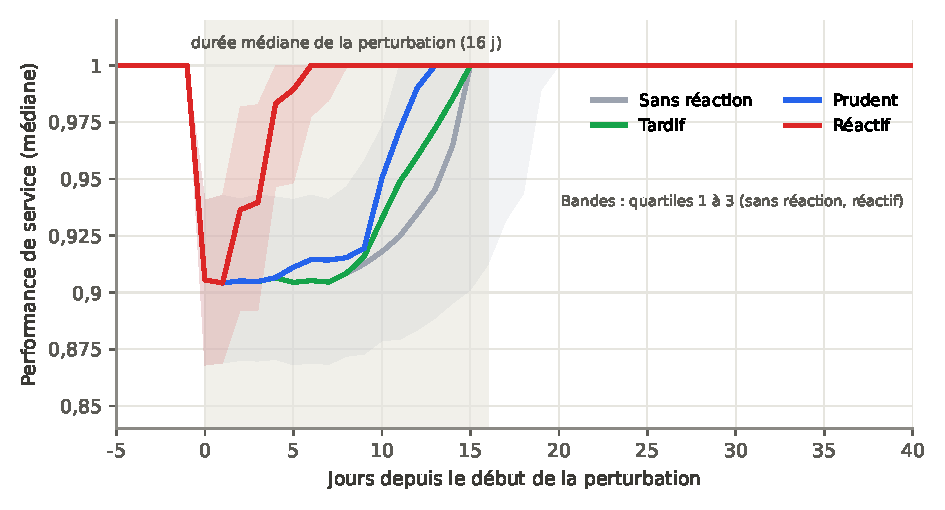
\includegraphics[width=\textwidth]{figures/Fig5_trajectoire_mediane.pdf}
\captionof{figure}{Trajectoire médiane de la performance selon la politique de gestion, sur les 2 000 crises de la base principale, recalées sur le début de la perturbation. Les bandes indiquent l'écart entre premier et troisième quartiles, sans réaction et sous le profil réactif.}\label{fig:d5}
\end{center}

Le troisième constat concerne le choix des leviers : le profil tardif n'engage que des leviers de demande, faute de pouvoir escalader au-delà de ses deux premiers choix pendant la crise, le profil prudent s'appuie surtout sur les stocks et la capacité additionnelle, le profil réactif sur le reroutage et la capacité. Leur efficacité dépend de la nature de la perturbation (tableau~\ref{tab:d13}).

\begin{table*}[htbp]
\caption{Réduction médiane de la perte cumulée par rapport à l'absence de réaction, selon la nature de la perturbation.}
\label{tab:d13}
\footnotesize
\begin{tabularx}{\textwidth}{@{}LLLL@{}}
\toprule
\textbf{Nature} & \textbf{Réactif} & \textbf{Prudent} & \textbf{Tardif} \\
\midrule
Panne fournisseur & 84 \% & 0 \% & 0 \% \\
Coupure de lien & 73 \% & 17 \% & 0 \% \\
Fermeture d'un site de stockage & 82 \% & 10 \% & 2 \% \\
Pic de demande & 87 \% & 23 \% & 13 \% \\
Congestion & 78 \% & 41 \% & 15 \% \\
\bottomrule
\end{tabularx}
\end{table*}

Le profil prudent est sans effet sur une panne fournisseur, que le déstockage ne compense pas, mais réduit de 41~\% la perte d'une congestion, choc diffus que des leviers globaux atténuent ; le profil réactif est le moins efficace face à une coupure de lien, dont les effets se propagent aux voies de secours.

Ces effets dessinent des contextes où une politique moins interventionniste suffit. En classant la perte cumulée en trois niveaux de même effectif, le profil prudent atteint le même niveau que le profil réactif dans 18~\% des crises, et le profil tardif dans 14~\%. Cette proportion atteint 31~\% pour les perturbations de 12 jours au plus, mais tombe à 11~\% au-delà de 18 jours : une crise courte peut être gérée sobrement, une crise longue exige de la réactivité. C'est cette dépendance au contexte que le réseau bayésien doit restituer (section~\ref{sec:6.3}).

Pour vérifier que ces résultats ne tiennent pas à la seule topologie d'ISOMORPH, un lot de contrôle de 500 scénarios a été généré sur le réseau paramétrique avec les mêmes réglages. Les crises y sont moins profondes (performance minimale médiane de 0,91) et l'ajustement moins bon, mais la perte cumulée reste très fidèle au service perdu (corrélation de 0,97). Les grandes proportions sont remarquablement stables : la part du service perdu évitée atteint 67~\%, 17~\% et 13~\% pour les profils réactif, prudent et tardif, contre 73~\%, 18~\% et 14~\% sur ISOMORPH. La topologie modifie en revanche l'efficacité des leviers selon la nature du choc : sur le réseau paramétrique, dont les voies de secours sont de faible capacité, le profil réactif ne réduit plus que de 25~\% la perte d'une coupure de lien et de 53~\% celle d'une fermeture, contre 73~\% et 82~\% sur ISOMORPH. L'effet d'une politique dépend donc conjointement de la nature du choc et de la redondance du réseau.

\subsection{Performance du réseau appris}
\label{sec:6.3}

Le réseau est appris sur 1 600 scénarios, soit 6 400 versions de crise, et évalué sur les 400 restants (section~\ref{sec:5.4}). La structure obtenue (Fig.~\ref{fig:d6}) compte 41 arcs, sans aucun arc contraire à l'ordre des paliers, et retrouve le mécanisme principal de la section~\ref{sec:6.2} : la perte cumulée dépend directement de la politique, de la profondeur $h$ et de la durée $d$ du palier dégradé, et cette durée dépend à son tour de la politique, de la durée de la perturbation et du délai de réaction. La politique agit donc sur la durée de la crise plutôt que sur sa profondeur. La nature de la perturbation conditionne les familles de leviers mobilisées ; la part des articles critiques reste isolée dans la plage étudiée.

\begin{center}
\fbox{\parbox{0.92\textwidth}{\footnotesize [FIGURE À INSÉRER. Source : BayesArtist, apprentissage du fichier \texttt{bayesartist\_apprentissage\_lotA.csv} avec les contraintes \texttt{bayesartist\_contraintes\_isomorph.json} (Greedy Hill Climbing, score BIC, lissage de Laplace), puis « Appliquer au canevas » avec paliers colorés. Contenu attendu : 20 nœuds et 41 arcs, disposés en cinq colonnes de gauche à droite (contexte, politique, réponse, mécanisme, résilience). Pour la lisibilité, mettre en évidence le chemin principal : profil vers $d$ (durée du palier dégradé) et vers IPC ; durée de la perturbation et délai de réaction vers $d$ ; $h$ et $d$ vers IPC. Si la capture reste trop dense, envoyer à Claude le fichier .bif pour une version redessinée.]}}
\captionof{figure}{Réseau bayésien appris sous contraintes, variables colorées par palier de l'ordre temporel d'une crise.}\label{fig:d6}
\end{center}

\begin{table*}[htbp]
\caption{Pronostic de la classe de perte cumulée sur les crises de test.}
\label{tab:d14}
\footnotesize
\begin{tabularx}{\textwidth}{@{}LLL@{}}
\toprule
\textbf{Modèle} & \textbf{Classement correct} & \textbf{Score de Brier} \\
\midrule
Distribution uniforme ou classe majoritaire & 34 \% & 0,667 \\
Politique de gestion seule & 60 \% & 0,494 \\
Réseau appris, contexte et politique & 65 \% & 0,466 \\
\bottomrule
\end{tabularx}
\end{table*}

Le pronostic, établi à partir des seules variables connues au moment de décider, classe correctement 65~\% des crises de test, contre 34~\% pour la classe majoritaire et 60~\% pour un modèle fondé sur la seule politique (tableau~\ref{tab:d14}). Le gain apporté par le contexte est réel mais modeste. La courbe d'apprentissage est presque plate, de 62,5~\% avec 200 scénarios à 63,7~\% avec 1 600 : la taille de la base n'est pas le facteur limitant, c'est l'information disponible au moment de décider. La perte dépend notamment de la tension du réseau, que le générateur n'exporte pas (section~\ref{sec:7.3}).

Le diagnostic est bien calibré pour la politique et la durée. Pour les crises de test à forte perte, la probabilité a posteriori de chaque politique (sans réaction, tardif, prudent, réactif) vaut 0,42, 0,32, 0,26 et 0,01, pour des fréquences observées de 0,41, 0,33, 0,26 et 0,005 ; celle d'une perturbation longue vaut 0,41, comme sa fréquence observée. Il l'est moins pour la nature du choc et la position de la cible : les crises touchant un point de passage obligé, 6~\% de la base, sont trop rares pour que le score retienne leurs effets propres.

La préconisation dépend de l'objectif fixé. Avec l'objectif d'une perte faible, seul le profil réactif l'atteint régulièrement, dans 90 \% des crises de test, et aucune autre politique ne réussit lorsqu'il échoue : la règle préconise alors toujours ce profil. Avec l'objectif moins exigeant d'une perte qui ne soit pas forte, un arbitrage apparaît entre sécurité et sobriété, que règle le seuil $\theta$ (tableau~\ref{tab:d15}). La référence a posteriori montre l'enjeu : dans 67 \% des crises de test, une politique plus sobre que le profil réactif aurait suffi, et dans 42 \% l'absence de réaction elle-même.

\begin{table*}[htbp]
\caption{Préconisation sur les crises de test, objectif d'une perte cumulée non forte.}
\label{tab:d15}
\footnotesize
\begin{tabularx}{\textwidth}{@{}LLL@{}}
\toprule
\textbf{Règle} & \textbf{Objectif atteint} & \textbf{Préconisations plus sobres que le profil réactif} \\
\midrule
Toujours le profil réactif & 99,2 \% & 0 \% \\
Réseau appris, $\theta$ = 0,9 & 99,2 \% & 0 \% \\
Réseau appris, $\theta$ = 0,8 & 97,5 \% & 15 \% \\
Réseau appris, $\theta$ = 0,7 & 86,2 \% & 37 \% \\
Réseau appris, $\theta$ = 0,6 & 69,5 \% & 84 \% \\
Référence a posteriori : politique la plus sobre ayant réussi & 99,2 \% & 67 \% \\
\bottomrule
\end{tabularx}
\end{table*}

Avec $\theta$ = 0,8, le réseau préconise une politique plus sobre dans environ une crise sur sept, pour un taux de réussite de 97,5 \%, soit moins de deux points sous la politique la plus interventionniste. À ce niveau d'exigence, la sobriété repose entièrement sur la durée prévue du choc : lorsque cette information est retirée de la description de la crise, la même règle ne préconise plus aucune politique sobre. Une estimation de la durée d'une perturbation a donc une valeur décisionnelle propre : elle permet d'économiser des leviers sans dégrader la résilience.

\subsection{Étude de cas illustrative}
\label{sec:6.4}

Deux crises de même nature illustrent l'usage du réseau. Dans la première, un site de stockage situé sur un point de passage obligé, comme l'entrepôt d'Atlanta, est fermé pour une longue durée. Le réseau (Fig.~\ref{fig:d7}) donne une probabilité de forte perte de 0,69 sans réaction, de 0,55 sous le profil tardif, de 0,44 sous le profil prudent et de 0,01 sous le profil réactif. Seul ce dernier atteint l'objectif avec une probabilité suffisante : la préconisation est sans ambiguïté, quel que soit le seuil retenu.

Dans la seconde, un site de stockage redondé est fermé pour une courte durée. La probabilité de forte perte tombe à 0,30 sans réaction, 0,22 sous le profil tardif et 0,20 sous le profil prudent. Avec $\theta$ = 0,8, le profil prudent atteint l'objectif avec une probabilité de 0,80 et devient la préconisation : face à un choc bref sur un site doublé, une réaction fondée sur le déstockage suffit, et mobiliser le reroutage et la capacité additionnelle n'apporterait qu'un gain marginal.

\begin{center}
\fbox{\parbox{0.92\textwidth}{\footnotesize [FIGURE À INSÉRER. Source : BayesArtist, réseau appris de la figure~\ref{fig:d6}, mode inférence. Évidences à poser : nature = \texttt{fermeture\_entrepot}, cible = \texttt{passage\_oblige}, duree = fort. Puis fixer successivement profil = none, tardif, prudent, reactif, et capturer la distribution du nœud IPC à chaque fois. Valeurs de contrôle pour la classe « fort » : 0,69, 0,55, 0,44 et 0,01. Présentation conseillée : les quatre captures assemblées côte à côte, ou une seule capture avec le profil réactif et les évidences visibles. Variante : Claude peut produire un diagramme en barres empilées des quatre distributions.]}}
\captionof{figure}{Pronostic de la perte cumulée selon la politique, pour la fermeture longue d'un site situé sur un point de passage obligé.}\label{fig:d7}
\end{center}

Le diagnostic éclaire le cas inverse, celui d'une crise à forte perte gérée par un profil prudent. Le réseau y associe une perturbation longue, avec une probabilité de 0,39 contre 0,33 a priori, un recours au déstockage presque certain (0,95) et une escalade jusqu'à trois leviers ou plus (0,40 contre 0,23 a priori). Il désigne ainsi une crise trop longue pour la politique choisie : le gestionnaire a escaladé, mais à partir de leviers de stock dont l'effet s'épuise, sans atteindre à temps le reroutage. Ce diagnostic oriente l'action corrective vers la politique, plus réactive ou dotée d'un autre ordre de leviers, plutôt que vers le réseau.

\subsection{Sensibilité à la couverture de stock}
\label{sec:6.5}

La représentation temporelle permet d'étudier le rôle des stocks, que la base principale neutralise. Sur le réseau ISOMORPH, avec ses délais de trajet d'origine, 60 crises ont été simulées pour chaque nature de perturbation et chaque couverture, sans réaction du gestionnaire, et l'on a compté celles qui produisent une baisse de service visible (Fig.~\ref{fig:d8} ; valeurs détaillées au tableau~S4 du matériel supplémentaire). La représentation par flux sert de référence.

\begin{center}
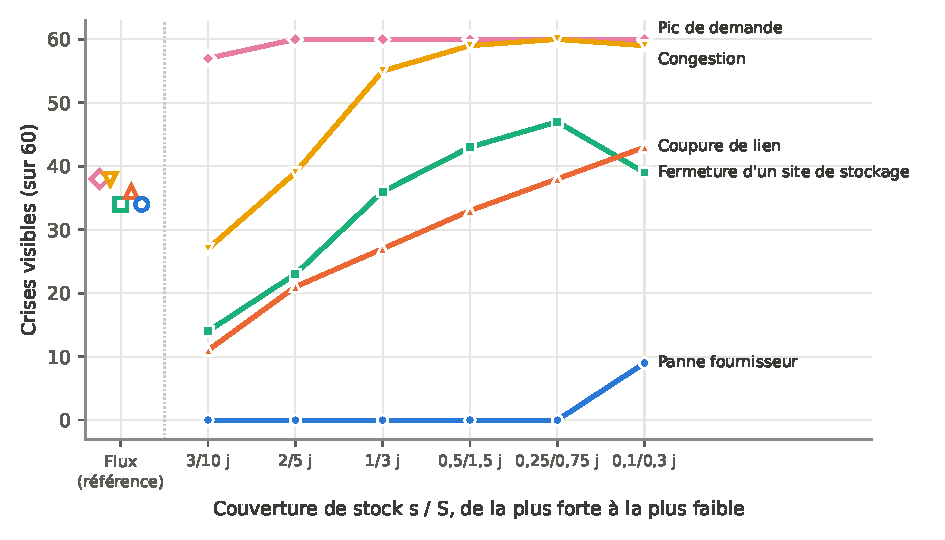
\includegraphics[width=\textwidth]{figures/Fig8_couverture_stock.pdf}
\captionof{figure}{Nombre de crises visibles sur 60 selon la couverture de stock, par nature de perturbation (réseau ISOMORPH, sans réaction). Les symboles creux, à gauche, donnent la référence de la représentation par flux.}\label{fig:d8}
\end{center}

Trois comportements se dégagent. Pour les ruptures de distribution, coupure de lien, fermeture d'un site de stockage et congestion, la couverture agit comme un levier de robustesse progressif : plus elle est faible, plus les crises visibles sont nombreuses, de 11 à 43 sur 60 pour une coupure de lien et de 27 à 59 pour une congestion. La frontière entre robustesse et résilience évoquée en section 4.4 se déplace donc de manière contrôlée avec le niveau de stock. Les pannes fournisseur sont au contraire absorbées dès que la couverture atteint un quart de jour, y compris pour des pannes de 15 à 60 jours à la couverture par défaut : la calibration de la demande borne le manque à servir pendant une panne, que quelques jours de stock suffisent à compenser. Enfin, le pic de demande est mieux absorbé sans stocks qu'avec : dans la représentation par flux, toute marge de capacité sert instantanément le surcroît de demande, alors qu'avec des délais, ce surcroît doit d'abord être prélevé sur des stocks dimensionnés sur le débit nominal, que le recomplètement ne reconstitue qu'après un délai.

La couverture de stock n'est donc pas un levier universel de résilience. Elle protège contre les pertes de capacité de distribution, est presque superflue contre une défaillance amont de faible ampleur, et ne protège pas contre un choc de demande, qui appelle des leviers de capacité ou de demande. Ces résultats, obtenus sans réaction du gestionnaire et à couverture uniforme, n'épuisent pas la question : l'interaction entre couverture et politique de gestion reste à étudier (section 7.3).

% Rapatrié depuis le doc de travail (onglet Article FR), révision 144.

\section{Discussion}
\label{sec:7}

\subsection{Apports théoriques}
\label{sec:7.1}

La première contribution est méthodologique. L'étude de la résilience pilotée bute sur l'absence de données reliant une perturbation, les décisions prises et la trajectoire de performance. La démarche proposée produit de telles données et leur donne une propriété que les données d'observation n'ont jamais : chaque crise y est observée sous plusieurs politiques, toutes choses égales par ailleurs. La politique devient ainsi une intervention au sens de \citet{pearl2009}, dont l'effet est identifiable par construction, et une préconisation peut être confrontée à ce qui se serait réellement produit.

La deuxième contribution porte sur la représentation de la résilience. Le triangle de résilience \citep{bruneau2003} et le profil de perturbation \citep{sheffi2005book} résument une crise par sa profondeur et sa durée. Les résultats montrent que ces deux dimensions ne relèvent pas des mêmes causes : la profondeur de la chute dépend surtout du choc, la gestion n'en modifie presque pas le minimum, alors que la durée de la crise dépend surtout de la gestion, le retour à la normale passant du quatorzième au quatrième jour selon la politique. Décomposer la trajectoire en paramètres de mécanisme, comme le fait la courbe hyperbolique composée, n'est donc pas un raffinement descriptif : c'est la condition pour attribuer une perte à sa cause. Le réseau appris retrouve d'ailleurs ce partage sans qu'il lui soit imposé.

La troisième contribution précise la typologie des stratégies d'atténuation et de contingence \citep{tomlin2006,chopra2004}. L'efficacité d'un levier n'est pas une propriété du levier, mais de sa rencontre avec la nature du choc et la topologie du réseau : le déstockage est sans effet sur une panne fournisseur mais atténue une congestion, l'efficacité de la réaction la plus rapide s'effondre lorsque les voies de secours sont étroites, et la couverture de stock protège contre les pertes de capacité de distribution sans protéger contre un choc de demande. Ces interactions plaident pour des règles de pilotage conditionnelles plutôt que génériques, que seul un modèle causal du réseau considéré permet d'établir.

\subsection{Implications managériales et économiques}
\label{sec:7.2}

Les indicateurs de résilience se traduisent directement en volume de ventes perdues. Sur le réseau ISOMORPH au niveau de tension étudié, une crise sans réaction coûte en médiane 1,34 jour de demande, soit environ 21 000 unités. Le profil réactif en évite en moyenne 1,06 jour, le profil prudent 0,34 et le profil tardif 0,22. Pour une marge unitaire m, la valeur d'une politique se lit donc comme le produit du service évité, de la demande journalière et de m, à comparer au coût des leviers qu'elle engage ; le modèle ne valorisant pas ce coût, cette comparaison revient au décideur, mais l'ordre de grandeur du gain est désormais connu.

Quatre implications managériales s'en dégagent. Premièrement, la vitesse de détection et de décision semble compter davantage que le choix des leviers : investir dans la surveillance de la performance et dans des délégations de décision pré-établies paraît prioritaire. Deuxièmement, l'information sur la durée prévisible d'un choc a une valeur économique propre : elle permet de gérer environ une crise sur sept avec une politique plus sobre, pour une perte de réussite inférieure à deux points, et la communication avec fournisseurs et transporteurs sur la durée des incidents mérite d'être organisée avant la crise. Troisièmement, les points de passage obligés réduisent l'efficacité de toute réaction et justifient des investissements de redondance ciblés, que les leviers de crise ne remplacent pas. Quatrièmement, les stocks de sécurité ne sont pas une protection universelle, et une réserve d'urgence gagne à être tenue séparée de la politique de commande, faute de quoi elle peut perturber le signal de réapprovisionnement (section~\ref{sec:3.5}).

\subsection{Limites et perspectives}
\label{sec:7.3}

Les résultats reposent sur des données simulées et en héritent les limites. Les valeurs posées faute de données de terrain, capacités, effets des leviers, caractéristiques des profils, ont été choisies pour être plausibles et sont toutes réglables, mais elles conditionnent les ordres de grandeur ; seules les tendances et les hiérarchies, stables entre les deux réseaux étudiés, doivent être généralisées. Le niveau de tension retenu et le relèvement des seuils de tolérance visent à produire des crises contrastées : ils ne décrivent pas une fréquence réelle de crises. Une validation sur des données d'entreprise, même partielles, reste nécessaire.

Plusieurs simplifications du gestionnaire simulé bornent la portée des préconisations. Les leviers n'ont pas de coût et restent engagés jusqu'à la fin de la période observée, ce qui rend la domination de la réactivité en partie structurelle ; introduire leur coût et leur levée transformerait la préconisation en arbitrage explicite entre coût et résilience. La nature de la perturbation est supposée diagnostiquée sans erreur, chaque scénario ne comporte qu'une perturbation, et la politique est représentée par le profil seul : en distinguer les composantes suppose des lots où elles varient indépendamment.

Le pronostic est limité par l'information disponible au moment de décider plutôt que par la taille de la base : la tension du réseau manque au contexte, et les crises touchant un point de passage obligé sont trop rares pour que leurs effets propres soient appris, ce qu'un échantillonnage stratifié corrigerait.

La représentation temporelle appelle enfin deux réserves. La couverture de stock est uniforme entre sites, et son interaction avec la politique de gestion n'a pas été étudiée. La recherche de la demande de référence par dichotomie suppose une monotonie qui n'est pas démontrée, même si la valeur retenue est toujours vérifiée par simulation.
% Rapatrié depuis le doc de travail (onglet Article FR), révision 144.

\section{Conclusion}
\label{sec:8}

Cet article a proposé une démarche en trois blocs pour étudier et piloter la résilience d'une chaîne logistique à partir de crises simulées. Un générateur soumet un réseau multi-échelon à des perturbations maîtrisées et rejoue chaque crise sous plusieurs politiques de gestion ; une courbe hyperbolique composée caractérise chaque trajectoire par des paramètres de mécanisme et des indicateurs de résilience ; un réseau bayésien causal, dont la structure respecte l'ordre temporel d'une crise et traite la politique comme une intervention, en tire pronostic, diagnostic et préconisation.

Appliquée au réseau ISOMORPH sur 2 000 crises, la démarche montre que la réaction des gestionnaires agit sur la durée d'une crise plutôt que sur sa profondeur : la politique la plus réactive évite 73 \% du service perdu, contre 18 \% et 14 \% pour les politiques prudente et tardive, une hiérarchie retrouvée sur un second réseau. L'efficacité de chaque politique dépend de la nature du choc et de la topologie, et la couverture de stock protège contre les ruptures de distribution mais pas contre les chocs de demande. Le réseau bayésien appris pronostique la classe de perte de 65 \% des crises nouvelles et préconise, lorsque la durée du choc est connue, une politique plus sobre dans environ une crise sur sept pour une perte de réussite inférieure à deux points.

La démarche est ouverte et transposable : tout réseau multi-échelon décrit dans le format proposé peut être étudié de la même façon. Trois prolongements en découlent directement : valoriser le coût des leviers pour arbitrer explicitement entre coût et résilience, imposer les leviers eux-mêmes pour en identifier l'effet causal propre, et confronter les préconisations à des crises réelles.

% Rapatrié depuis le doc de travail (onglet Article FR), révision 144.

\section*{Disponibilité des données}

[La base de scénarios et le générateur seront déposés dans un entrepôt public ; lien et DOI à ajouter, anonymisés pour l'évaluation.]

\section*{Déclaration d'usage de l'IA générative}

Pendant la préparation de ce travail, les auteurs ont utilisé Claude (Anthropic) pour rédiger et structurer une partie du texte. Google AI Studio a été utilisé pour appuyer le développement des deux applications BayesArtist et Isomorph-Reborn. Après usage de ces outils, les auteurs ont relu et modifié le contenu autant que nécessaire, ils ont vérifié durant et après le développement des applications pour confirmer la correspondance exacte avec le cahier des charges et les descriptions donnés dans le présent papier. Les auteurs assument ainsi l'entière responsabilité du contenu de l'article. 
% Déclaration des contributions selon la taxonomie CRediT.
% En évaluation en double aveugle, mettre \anonymetrue dans sc_reborn_ijpe.tex :
% la déclaration n'est alors pas imprimée et doit figurer sur la page de titre séparée.
\ifanonyme\else
\section*{Contribution des auteurs (CRediT)}

\textbf{Naïma Rahiel :} Conceptualization, Methodology, Formal analysis, Validation, Writing -- original draft, Writing -- review \& editing.
\textbf{Sid-Ali Addouche :} Conceptualization, Methodology, Software, Investigation, Data curation, Formal analysis, Visualization, Writing -- original draft, Writing -- review \& editing, Supervision, Project administration, Funding acquisition.
\textbf{El Mouloudi Dafaoui :} Writing -- review \& editing.
\textbf{Abderrahman El Mhamedi :} Writing -- review \& editing.
\textbf{Saïd Amari :} Writing -- review \& editing.
\textbf{Agnès Letouzey :} Writing -- review \& editing.
\textbf{Xavier Desforges :} Writing -- review \& editing.
\textbf{Kamal Medjaher :} Writing -- review \& editing.
\fi


\bibliographystyle{cas-model2-names}
\bibliography{references}

% ---------------------------------------------------------------------
% LISTE DE SUIVI DES DÉPÔTS (à retirer avant la soumission)
% ---------------------------------------------------------------------
\noindent{\color{blue}\fbox{\parbox{0.96\textwidth}{\footnotesize
\textbf{Liste de suivi des dépôts (à retirer par toi ou moi avant la soumission).} La politique de données d'IJPE (option C) impose le dépôt des données dans un entrepôt et une déclaration de disponibilité dès la soumission ; les fichiers supplémentaires doivent être téléversés avec le manuscrit, chacun avec une légende courte, et ne peuvent plus être ajoutés qu'à l'étape de révision.
\begin{itemize}[leftmargin=1.2em, itemsep=1pt]
\item[$\boxtimes$] \textbf{Mendeley Data} (fait, en brouillon) : le jeu de données contient, pour chaque lot (A : réseau ISOMORPH, tension 75, 2 000 scénarios ; B : réseau paramétrique, 500 scénarios) : \texttt{hypotheses\_lot\_A\_isomorph\_tension75.json}, \texttt{hypotheses\_lot\_B\_parametrique\_tension75.json}, les fichiers des lots complémentaires C0 et C1 (\texttt{hypotheses\_lot\_C0\_sans\_perturbation.json}, \texttt{hypotheses\_lot\_C1\_perturbation\_mineure.json} et leurs exports), \texttt{reseau\_isomorph-originel.json}, \texttt{ip\_timeseries.csv}, \texttt{resilience\_ip.csv}, les fichiers de scénarios, de perturbations et de décisions, la base \texttt{rb\_training\_42\_*.csv}, \texttt{bayesartist\_apprentissage\_lotA.csv}, \texttt{bayesartist\_contraintes\_isomorph.json} et le réseau appris au format \texttt{.bif}.
\item[$\boxtimes$] Rédiger le README du jeu de données : contenu de chaque fichier, signification des colonnes, graine et configuration de génération, correspondance avec les tableaux et figures de l'article.
\item[$\square$] Choisir la licence des données (CC-BY 4.0 conseillée) ; garder le jeu de données privé pendant l'évaluation et générer le lien de partage réservé aux relecteurs.
\item[$\boxtimes$] \textbf{Isomorph-Reborn} : déposé dans le même jeu de données Mendeley (pas de Zenodo) ; vérifier la licence du code (MIT conseillée), le manuel d'utilisation et le README d'installation.
\item[$\boxtimes$] README propre d'Isomorph-Reborn (installation, aucune clé requise, Firebase facultatif) ; \texttt{firebase-applet-config.json} retiré du code déposé ; fichiers renommés selon le README du jeu de données.
\item[$\square$] Choisir la licence du code d'Isomorph-Reborn (MIT conseillée) et la reporter dans son README.
\item[$\boxtimes$] Lot C0 : \texttt{resilience\_ip} réexporté.
\item[$\square$] Vérifier que le manuel d'utilisation est à jour (correctif de la représentation temporelle) et qu'il décrit les manœuvres citées dans les consignes de reproductibilité des figures.
\item[$\square$] Pour l'évaluation anonyme : fournir un lien anonymisé vers le code (par exemple anonymous.4open.science) ou une archive jointe réservée aux relecteurs.
\item[$\square$] \textbf{BayesArtist} : non diffusé ; vérifier que la base CSV et le fichier de contraintes suffisent à reproduire l'apprentissage dans un outil tiers (essai conseillé avec bnlearn ou pgmpy).
\item[$\boxtimes$] \textbf{Matériel supplémentaire} : \texttt{sc\_reborn\_supplementaire.tex} compilé (S0 à S3, figure S1, tableaux S1 à S4).
\item[$\square$] Rédiger la légende courte du matériel supplémentaire et le téléverser avec le manuscrit.
\item[$\square$] À l'acceptation : publier le jeu de données, vérifier que son DOI est bien \acompleter{10.17632/jm2phpyw92.1} dans la bibliographie, que les auteurs de la référence (Addouche et Rahiel) correspondent à ceux du dépôt, et retirer le lien de consultation privé.
\item[$\square$] Renseigner la déclaration de disponibilité des données dans le formulaire de soumission.
\item[$\boxtimes$] Déclaration CRediT rédigée (section en fin d'article) ; financement avec le numéro de convention ANR-21-CE10-0020.
\item[$\square$] \textbf{Exigences de soumission Elsevier} : fournir les points clés dans un fichier séparé ; ajouter les identifiants ORCID ; confirmer la déclaration d'intérêts ; vérifier le mode d'évaluation (anonymat simple ou double) et, s'il est double, déplacer le financement et les remerciements sur une page de titre séparée.
\item[$\square$] Ramener le manuscrit vers environ 10 000 mots (environ 13 000 actuellement, tableaux et légendes compris), par exemple en déplaçant les consignes de reproductibilité des figures dans le matériel supplémentaire.
\item[$\boxtimes$] Référence Rajah et al. (2025) ajoutée à l'état de l'art.
\item[$\square$] Traduire l'article en anglais (texte, figures, tableaux et matériel supplémentaire).
\end{itemize}}}}

% Matériel supplémentaire, reproduit à la fin du PDF de l'article
% (il est aussi compilé seul par sc_reborn_supplementaire.tex pour la soumission).
\clearpage
\begin{center}{\Large\bfseries Matériel supplémentaire}\end{center}
\setcounter{table}{0}
\renewcommand{\thetable}{S\arabic{table}}
\setcounter{figure}{0}
\renewcommand{\thefigure}{S\arabic{figure}}
% Corps du matériel supplémentaire, partagé par sc_reborn_supplementaire.tex
% (fichier séparé pour la soumission) et sc_reborn_ijpe.tex (annexé à la fin de l'article).

\section*{S0. Vue détaillée de la démarche}

La figure~\ref{fig:S1} détaille la démarche résumée à la figure 1 de l'article. Pour chacun des trois blocs, elle précise les données d'entrée, les traitements et les sorties : la génération des crises étiquetées et de leurs quatre versions (simuler), l'ajustement de la courbe de résilience et le calcul des indicateurs (mesurer), puis l'apprentissage du réseau bayésien causal et ses trois usages (apprendre). Des vignettes illustrent une trajectoire, une courbe ajustée et la structure du réseau appris.

\begin{center}\begin{minipage}{\textwidth}\centering
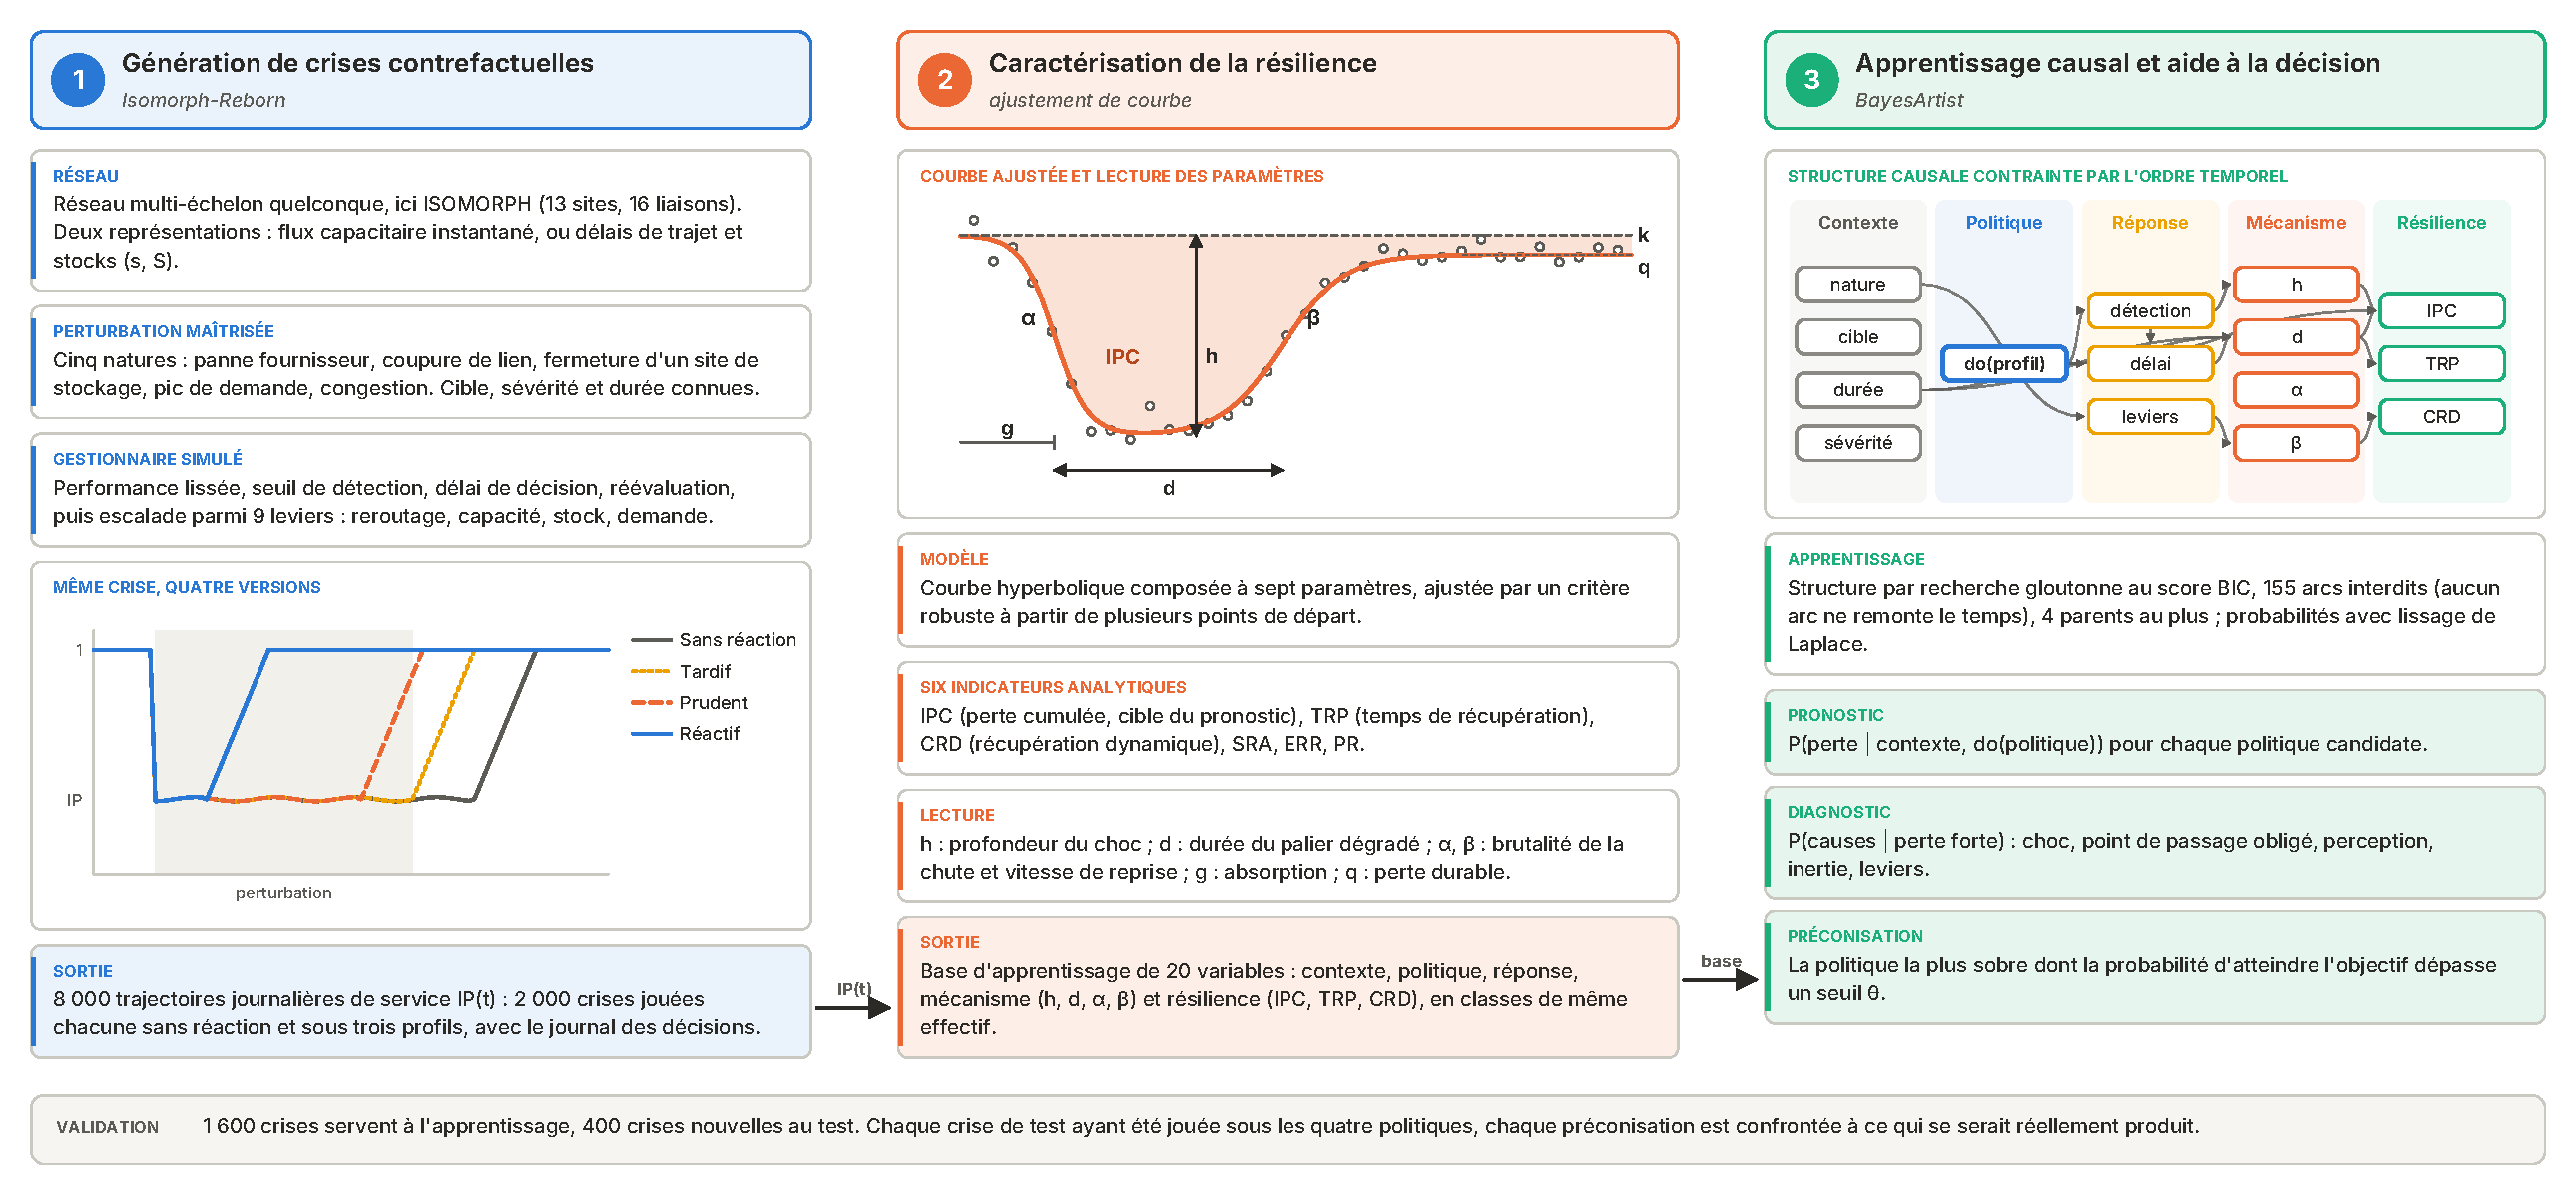
\includegraphics[width=\textwidth]{figures/Fig1_demarche.pdf}
\captionof{figure}{Démarche détaillée en trois blocs : entrées, traitements et sorties de chaque bloc.}\label{fig:S1}
\end{minipage}\end{center}

\section*{S1. Compléments sur le générateur de scénarios (Simuler)}

Cette partie reprend les détails de modélisation retirés de la section 3 de l'article pour respecter la longueur demandée par la revue.

\subsection*{Positionnement par rapport à ISOMORPH}

Le tableau~\ref{tab:S1} résume les écarts entre la démarche proposée et le jumeau numérique ISOMORPH.

\begin{center}\begin{minipage}{\textwidth}
\captionof{table}{Positionnement de la démarche par rapport à ISOMORPH.}
\label{tab:S1}
\footnotesize
\begin{tabularx}{\textwidth}{@{}LLL@{}}
\toprule
\textbf{Dimension} & \textbf{ISOMORPH} & \textbf{Démarche proposée} \\
\midrule
Réseau & 13 nœuds, destination unique, pas journalier & Réseau multi-échelon quelconque ; réseau paramétrique à redondance partielle et réseau ISOMORPH d'origine comme références \\
Dynamique & Stocks gérés en (s, S) & Deux représentations emboîtées : flux capacitaire instantané, ou délais de trajet et de production avec stocks (s, S) à couverture réglable \\
Perturbations & Aléatoires, non étiquetées & Cinq natures maîtrisées : cible, date, durée et sévérité connues \\
Décisions & Paramètres fixés avant la simulation & Gestionnaire simulé réagissant en cours de crise \\
Expérimentation & Tirages indépendants & Même crise rejouée sous plusieurs comportements de gestion \\
\bottomrule
\end{tabularx}
\end{minipage}\end{center}

\subsection*{Réseaux de référence}

Deux réseaux servent de référence (tableau~\ref{tab:S2}). Le réseau paramétrique comporte trois échelons : trois usines, neuf entrepôts et un client final. Chaque entrepôt est approvisionné par une usine principale, par une usine de secours via un lien de moindre capacité et, pour un entrepôt sur trois, par une troisième usine. La redondance est donc partielle par construction : la perte de la voie principale d'un entrepôt ne peut être que partiellement compensée par ses voies de repli, comme dans la plupart des réseaux réels où la double source reste coûteuse.

Le réseau ISOMORPH reprend la topologie d'origine (Fig.~3 de l'article) : treize villes reliées par seize liaisons, avec un hub et cinq échelons intermédiaires entre les sources et le client. Le fichier d'origine ne fixant pas toutes les grandeurs nécessaires, trois hypothèses complètent sa description. La capacité de chaque liaison est tirée à plus ou moins 10 \% autour de sa valeur d'origine. La capacité de production de chaque source est fixée à 0,8 fois la capacité cumulée de ses liaisons sortantes : à 1,0, la production ne pourrait jamais constituer un goulot et le report de charge vers les sites de production sains serait sans effet. Le dernier kilomètre est enfin supposé illimité ; les deux derniers sites de stockage avant le client n'ont alors ni capacité propre ni liaison sortante limitée, et échappent aux leviers d'expédition.

Les valeurs nominales des deux réseaux figurent au tableau~\ref{tab:S2}.

\begin{center}\begin{minipage}{\textwidth}
\captionof{table}{Caractéristiques des deux réseaux de référence (valeurs nominales).}
\label{tab:S2}
\footnotesize
\begin{tabularx}{\textwidth}{@{}LLL@{}}
\toprule
\textbf{Élément} & \textbf{Réseau paramétrique} & \textbf{Réseau ISOMORPH} \\
\midrule
Sites et échelons & 3 usines, 9 entrepôts, 1 client & 13 villes, 16 liaisons, 1 hub, 5 échelons intermédiaires \\
Capacité de production d'une source (unités par jour) & 200 à 320 & 0,8 fois la capacité de ses liaisons sortantes \\
Capacité des liaisons (unités par jour) & Voie principale 60 à 110 ; voie de secours 15 à 35 ; troisième voie 10 à 20 & Valeur d'origine $\pm$ 10 \% ; dernier kilomètre illimité \\
Capacité d'expédition d'un site de stockage (unités par jour) & 50 à 100 & Portée par les liaisons sortantes \\
Délai de trajet, représentation temporelle (jours) & 0 par défaut, réglable & 1 à 8 (valeurs d'origine) \\
Délai de production, représentation temporelle (jours) & 0 par défaut, réglable & 0 par défaut, réglable \\
Part des articles critiques dans la demande & 15 \% à 45 \% & 15 \% à 45 \% \\
Fluctuation journalière de la demande & $\pm$ 3 \% à $\pm$ 8 \% & $\pm$ 3 \% à $\pm$ 8 \% \\
\bottomrule
\end{tabularx}
\end{minipage}\end{center}

\subsection*{Règles de la représentation temporelle}

Trois règles complètent la représentation. Chaque jour, un site de stockage sert d'abord les besoins du jour, puis le recomplètement des sites en aval, et la répartition privilégie la liaison principale avant les liaisons de secours. Les articles critiques et ordinaires sont agrégés dans les stocks, la priorité aux articles critiques ne s'appliquant qu'au service du client. Enfin, les liaisons vers le client sont servies le jour même : avec un délai sur ces liaisons, le client recevrait aujourd'hui ce qu'il a commandé la veille, et l'indicateur baisserait à chaque hausse de la demande d'un jour à l'autre, même sans perturbation ; il mesurerait alors le bruit de la demande et non la disponibilité du réseau.

Avant toute observation, le réseau est simulé sans perturbation pendant une pré-chauffe de 60 jours, qui amène les stocks et la matière en route à leur régime établi. Cette pré-chauffe est commune aux quatre versions d'une même crise (section 3.6 de l'article).

Les deux représentations sont emboîtées. À délais nuls, la représentation temporelle reproduit presque exactement la représentation par flux : l'écart moyen de l'indicateur de performance reste compris entre 0,00025 et 0,002 selon les cas testés. Avec des délais, en revanche, les stocks modifient profondément la réponse du réseau aux chocs, dans une mesure qui dépend de la couverture et de la nature du choc ; la section 6.5 de l'article en analyse la sensibilité.

\subsection*{Calibration de la demande de référence}

Dans la représentation par flux, le volume livrable $F(t)$ d'un jour est la quantité maximale que le réseau peut acheminer des sources au client compte tenu de toutes ses capacités, dégradées ou renforcées ce jour-là. Cette formulation fait apparaître naturellement les goulots d'étranglement : c'est souvent la capacité d'expédition des sites de stockage, et non la production, qui limite le service. Dans la représentation temporelle, $F(t)$ désigne le volume que la circulation de la matière et les stocks permettent effectivement de livrer ce jour-là (section 3.3 de l'article). Dans les deux cas, ce volume sert en priorité les articles critiques, et la performance du jour est mesurée par un taux de service pondéré, dans lequel les articles critiques comptent triple :

Dans la représentation temporelle, $F_{\mathrm{inc}}$ et $F_{\mathrm{nom}}$ sont les volumes que la circulation de la matière permet effectivement d'écouler, au plus égaux au volume maximal de la représentation par flux. Le second terme ne suffit plus à garantir l'absence de dégradation : les recomplètements par à-coups et les délais peuvent laisser une demande non servie un jour donné, même sans perturbation. La demande de référence est donc vérifiée par simulation. Chaque scénario est simulé sans perturbation, pré-chauffe comprise, avec sa propre série de fluctuations, et $D_{0}$ est la plus grande demande entière au plus égale à $D_{\mathrm{max}}$ qui est servie intégralement chaque jour :

$\mathrm{IP}_{d}(t)$ désigne l'indicateur de performance obtenu sous une demande de référence $d$, les niveaux s et S étant recalculés par l'équation~(2) de l'article pour chaque demande essayée. La recherche procède par dichotomie sur les entiers et ne fait qu'abaisser $D_{\mathrm{max}}$ ; la valeur retenue est toujours vérifiée par simulation. Lorsque même une demande d'une unité n'est pas servie intégralement, la couverture de stock est trop faible au regard des fluctuations et des délais : le scénario n'admet aucun régime nominal sans dégradation, et le plan d'expériences est refusé plutôt que poursuivi avec une demande arbitraire. Cette condition de faisabilité relie directement la couverture de stock, les délais d'approvisionnement et la variabilité de la demande.

\subsection*{Leviers de stock en représentation temporelle}

Dans la représentation temporelle, les deux leviers de stock changent de mécanisme. Le pré-positionnement (D7) relève temporairement les niveaux s et S des sites de stockage et déclenche une commande immédiate. Le déstockage (D6) libère une réserve de sécurité tenue à l'écart du stock ordinaire : elle n'est pas visible de la politique de commande et ne sert que la demande que le stock ordinaire n'a pu satisfaire.

Ce choix n'est pas anodin. Injectée directement dans le stock ordinaire, la même quantité faisait passer certains sites au-dessus de leur point de commande. Ils sautaient alors un recomplètement, le besoin manquant remontait jusqu'aux sources, qui restaient à l'arrêt un jour de panne, et la capacité de production ainsi perdue ne se rattrapait pas : sur un cas mesuré, le levier réduisait le volume livré au lieu de l'accroître. Une intervention d'urgence sur les stocks peut donc perturber le signal de réapprovisionnement qu'elle devait soulager. La réserve séparée garantit que le déstockage ne réduit jamais le volume livré. Les deux leviers de stock excluent enfin les sites de stockage sans capacité propre et à liaisons sortantes illimitées, sur lesquels ils n'ont pas de prise (section 3.2 de l'article).

\subsection*{Niveau de tension et contenu des observations}

Toutes les valeurs posées par hypothèse faute de données de terrain peuvent être modifiées : capacités, effets des leviers, caractéristiques des profils, hypothèses qui complètent le réseau ISOMORPH et paramètres de la représentation temporelle. Pour explorer des contextes contrastés, un niveau de tension global, de 0 à 100, déplace simultanément quatre groupes d'hypothèses : l'intensité et la durée des chocs, la tension du réseau, l'efficacité des leviers et la réactivité des gestionnaires. Le niveau 50 correspond aux valeurs nominales présentées ici. Le niveau 0 décrit un réseau surcapacitaire soumis à des chocs brefs et géré par des décideurs très réactifs ; le niveau 100 décrit des chocs de 12 à 32 jours sur un réseau saturé, avec des leviers peu efficaces et des délais de décision allant jusqu'à 12 jours. Lorsque le réseau est imposé, ce niveau continue de piloter la sévérité et la durée des chocs, la tension entre demande et capacité, l'efficacité des leviers et la réactivité des gestionnaires, mais ne modifie pas les capacités du réseau, qui viennent de sa description. Il ne touche pas non plus aux délais ni à la couverture de stock, qui relèvent de la représentation du réseau et non de l'intensité de la crise.

Chaque version d'une crise constitue une observation complète, qui réunit le contexte du réseau (identité et taille du réseau, demande de référence, part des articles critiques), la perturbation subie, le journal des décisions (date de détection, leviers mobilisés et dates d'engagement) et la trajectoire journalière de performance. Les niveaux de stock et la matière en route ne sont pas enregistrés : la base décrit une crise par ses causes, ses décisions et le service rendu, et non par l'état interne du réseau. Des grandeurs descriptives simples, performance minimale, performance cumulée perdue et délai de retour à la normale, servent au contrôle de la base. La caractérisation de la résilience proprement dite est confiée au bloc 2.

\section*{S2. Signatures des dysfonctionnements sur la courbe de résilience}

Les paramètres de la courbe relient la trajectoire observée aux mécanismes décrits en section 3 de l'article. Le tableau~\ref{tab:S3} résume les signatures attendues ; il constitue un ensemble d'hypothèses que l'analyse des résultats et l'apprentissage causal permettent de confirmer ou de nuancer.

\begin{center}\begin{minipage}{\textwidth}
\captionof{table}{Signatures des dysfonctionnements sur la courbe de résilience.}
\label{tab:S3}
\footnotesize
\begin{tabularx}{\textwidth}{@{}LLL@{}}
\toprule
\textbf{Phénomène} & \textbf{Signature attendue sur la courbe} & \textbf{Origine probable} \\
\midrule
Absorption du choc & $h$ faible, $g$ élevé & Marges de capacité, voies de secours suffisantes \\
Absorption par les stocks & $h$ faible ou nul, $g$ élevé & Couverture de stock élevée au regard de la durée du choc \\
Rupture brutale & $h$ élevé, $\alpha$ élevé & Coupure ou fermeture sévère, réseau sous tension \\
Rupture différée & $g$ élevé, puis $h$ élevé & Stocks épuisés en cours de crise, matière en route insuffisante \\
Dégradation progressive & $\alpha$ faible & Congestion diffuse, pic de demande modéré \\
Crise prolongée & $d$ élevé & Perturbation longue, détection tardive, inertie décisionnelle \\
Reprise retardée & $d$ supérieur à la durée du choc & Reconstitution des stocks et de la matière en route après le retour des capacités \\
Reprise rapide & $\beta$ élevé, TRP faible & Levier efficace engagé tôt \\
Perte durable & $q$ $<$ 0 & Capacité non restaurée à la fin de la période, stock épuisé \\
Sur-récupération & $q$ $>$ 0 & Leviers maintenus après la fin de la perturbation \\
\bottomrule
\end{tabularx}
\end{minipage}\end{center}

\section*{S3. Sensibilité à la couverture de stock : valeurs détaillées}

Le tableau~\ref{tab:S4} donne les valeurs représentées à la figure 10 de l'article.

\begin{center}\begin{minipage}{\textwidth}
\captionof{table}{Crises produisant une baisse de service visible, sur 60, selon la couverture de stock (réseau ISOMORPH, sans réaction).}
\label{tab:S4}
\footnotesize
\begin{tabularx}{\textwidth}{@{}LLLLLLLL@{}}
\toprule
\textbf{Nature} & \textbf{Flux} & \textbf{3 / 10 j} & \textbf{2 / 5 j} & \textbf{1 / 3 j} & \textbf{0,5 / 1,5 j} & \textbf{0,25 / 0,75 j} & \textbf{0,1 / 0,3 j} \\
\midrule
Panne fournisseur & 34 & 0 & 0 & 0 & 0 & 0 & 9 \\
Coupure de lien & 36 & 11 & 21 & 27 & 33 & 38 & 43 \\
Fermeture d'un site de stockage & 34 & 14 & 23 & 36 & 43 & 47 & 39 \\
Pic de demande & 38 & 57 & 60 & 60 & 60 & 60 & 60 \\
Congestion & 38 & 27 & 39 & 55 & 59 & 60 & 59 \\
\bottomrule
\end{tabularx}
\end{minipage}\end{center}


\end{document}
